%% main.tex — MSc thesis (Cranfield CUThesis2026 template)
%% Author: Biswajeet Panda
%% Compile on Overleaf (TeXLive 2024/2025) — CUThesis2026.sty needs the
%% tagging / pdfmanagement packages. Build order: pdflatex -> bibtex -> pdflatex x2.
%%
%% >>> VERIFY the metadata below against your programme handbook before submission. <<<

\DocumentMetadata{tagging=on,
    tagging-setup={math/setup=mathml-SE},
    pdfstandard=ua-2,
    pdfstandard=a-4f,
    lang=en-UK
}

\documentclass[12pt,oneside]{book}

\usepackage{CUThesis2026}
\usepackage{lscape}
\usepackage{booktabs}   % nicer tables
\usepackage{siunitx}    % \SI units

% Numbered (Cranfield Numbered / Vancouver-style) referencing via biblatex.
% 'sorting=none' numbers references in order of first appearance. Overleaf runs
% biber automatically. \parencite -> "[n]" and \textcite -> "Author et al. [n]".
\usepackage{csquotes}
\usepackage[style=numeric-comp,sorting=none,backend=biber]{biblatex}
\addbibresource{references.bib}

% Times New Roman: the template loads mathptmx, which sets the serif font to
% Times (the pdfLaTeX-standard equivalent of Times New Roman) for text and maths.
% Leaving the sans-serif override commented out therefore gives a Times document.
% \renewcommand{\familydefault}{\sfdefault} % (commented: use Times, not sans-serif)

% ---- Title-page metadata (VERIFY) --------------------------------------------
\title{Mobile Manipulator Grasping of Everyday Objects Using Vision--Language--Action Models}
\author{Biswajeet Panda}
\date{September 2026}
\faculty{\FEAS}
\course{Robotics}
\degree{MSc}
\supervisors{Dr Gilbert Tang and Prof Phil Webb}
\academicyear{2025--2026}
\copyrightyear{2026}

\copyrightinstructions{(NB. Please refer to the \href{https://www.cranfield.ac.uk/-/media/files/rio/research-related-policies/intellectual-property-policy.ashx?la=en&hash=A1E0318F44085380F86D3B32BEB1B1FA0532A615}{Intellectual Property Policy} for full details on intellectual property and copyright ownership.)}

\begin{document}

\frontmatter
\maketitle

% ---- Abstract (<= 300 words) -------------------------------------------------
\begin{abstract}
Vision–Language–Action (VLA) models promise generalist robot control by extending a pretrained vision–language backbone to output robot actions, letting a single network handle perception, language understanding and manipulation together. But state-of-the-art VLAs are large, and it is not obvious that a capable one can be fine-tuned and deployed on a single consumer GPU — or that "capable" means what it appears to. This thesis investigates both questions through a language-driven supermarket task, built in the MuJoCo physics simulator, in which a mobile manipulator must pick a named grocery item from a shelf and place it in a basket.

A preliminary study on the RoboCasa kitchen benchmark found that small, deployable models failed outright, even after fine-tuning — a result that could easily have ended the project. Instead it motivated a deliberate change of strategy: rather than chase a harder benchmark with a bigger model, build a controlled task and get the methodology right first. The compact SmolVLA model is fine-tuned by freezing its pretrained vision–language backbone and training only the action expert, comfortably within a 12 GB budget, on a modest set of scripted-expert demonstrations. The resulting policy is, by the usual measure, a success: it completes the task reliably, and a documented failure analysis shows how an initial 0\% placement rate was traced to a specific, fixable defect rather than a fundamental one.

The more interesting story begins after that success is established. A series of controlled interventions probes what the policy has actually learned, and the answer is not the one the headline number suggests. The policy is genuinely language-conditioned — naming a different item sends the arm somewhere different — but displacing the items from their trained positions reveals that this conditioning is recall, not perception: the policy reaches for where an item used to be, never for where it actually is. A small non-language policy, trained on the same data, matches its manipulation quality on the item tested. The apparent intelligence of the system, in other words, is doing less work than it appears to.

Read together, these results argue that at this scale of data and hardware, the discipline of evaluation — testing a model past the point where it looks like it works — matters more than the scale of the model itself, and that a compact VLA is a genuinely practical choice for constrained deployment provided its operating conditions, and its limits, are stated honestly rather than assumed.

\end{abstract}

\begin{keywords}
Robot learning; Imitation learning; Mobile manipulation; Flow-matching policy;
MuJoCo simulation; Language-conditioned grasping.
\end{keywords}

% ---- Acknowledgements --------------------------------------------------------
\chapter{Acknowledgements}
I would like to thank my supervisors, Dr Gilbert Tang and Prof Phil Webb, for
their guidance and support throughout this project. I am also grateful to the
open-source robotics community --- in particular the developers of MuJoCo,
robosuite, the MuJoCo Menagerie and Hugging Face LeRobot --- whose tools and
model checkpoints made this work possible.

{
\clearpage
\singlespacing
{\tableofcontents}
\clearpage
\listoffigures
\clearpage
\listoftables
}

% ---- Abbreviations -----------------------------------------------------------
\begin{listofabbreviations}
    \abbrev{VLA}{Vision--Language--Action model}
    \abbrev{VLM}{Vision--Language Model}
    \abbrev{LLM}{Large Language Model}
    \abbrev{ACT}{Action Chunking Transformer}
    \abbrev{IK}{Inverse Kinematics}
    \abbrev{DOF}{Degree of Freedom}
    \abbrev{GPU}{Graphics Processing Unit}
    \abbrev{VRAM}{Video Random-Access Memory}
    \abbrev{CI}{Confidence Interval}
    \abbrev{RL}{Reinforcement Learning}
    \abbrev{RGB}{Red--Green--Blue (colour image)}
    \abbrev{EGL}{Embedded-System Graphics Library (headless OpenGL context)}
    \abbrev{FEAS}{Faculty of Engineering and Applied Sciences}
\end{listofabbreviations}

% ---- Main matter -------------------------------------------------------------
\mainmatter
\pagestyle{fancy}
\fancyhead[L]{\nouppercase{\leftmark}}
\fancyhead[R]{\nouppercase{\rightmark}}

\chapter{Introduction}
\label{chap:intro}

\section{Motivation}
\label{sec:motivation}
Retrieving items from a shopping list is a deceptively difficult robotics task.
It requires three capabilities at once: \emph{perception}, to see and identify
the correct object among clutter on a shelf; \emph{language understanding}, to
determine which item a natural-language request refers to; and
\emph{manipulation}, to physically grasp the object and place it accurately in a
receptacle. Traditionally, each of these is addressed by a separate, hand-engineered
subsystem, and integrating them is brittle and labour-intensive.

The task is also of practical interest. Service and retail robotics --- stocking
shelves, fulfilling orders, assisting shoppers --- is a rapidly growing application
area in which robots must operate in unstructured, human-centric environments and
respond to natural requests. A robot that can be told, in ordinary language, what to
fetch, and that can then perceive and manipulate everyday products, is a building
block for such applications. Studying this capability in simulation, under a tight
hardware budget, is a way to understand what is achievable with accessible resources
before committing to expensive hardware and data collection.

Vision--Language--Action (VLA) models offer an appealing alternative. By taking a
vision--language backbone that has already learned to perceive images and follow
language, and extending its output space from text to robot actions, a
\emph{single} network can map camera images and an instruction directly to motor
commands \parencite{zitkovich2023rt2, sapkota2026vla}. This promises generalist
robot control without a bespoke pipeline for every object and instruction.

The practical obstacle is scale. Capable VLAs typically contain billions of
parameters and are trained and deployed on large accelerators. For a student or a
low-cost robot, the relevant question is not ``what is the largest possible
model?'' but ``\emph{what can be fine-tuned and run on a single consumer GPU?}''
This thesis takes that constraint seriously --- a 12~GB GPU --- and asks whether a
compact VLA can nonetheless perform a useful, language-driven manipulation task
reliably.

The constraint is not merely a matter of convenience. It changes the design space:
it rules out the largest and most capable models, forces a choice about which parts
of a pretrained network to adapt, and makes data efficiency and evaluation
discipline decisive rather than optional. A recurring finding in this thesis, and in
the recent literature, is that under such constraints the quality of the data and of
the evaluation matters more than the raw capacity of the model. The work is
therefore as much about \emph{methodology} --- how demonstrations are collected, how
success is defined and measured, and how a deployment checkpoint is chosen --- as it
is about the model itself.

\section{Problem statement and scope}
\label{sec:problem}
The task studied in this thesis is a language-conditioned pick-and-place in a
simulated supermarket. A mobile manipulator --- a UR10e arm mounted on an Omron
mobile base, fitted with a Robotiq two-finger gripper --- is given a text
instruction naming a grocery item (for example, ``pick up the milk carton and
place it in the basket''). It must locate that item on a shelf, grasp it, and
place it in an onboard basket. The work is conducted entirely in the MuJoCo
physics simulator, which provides a safe, reproducible and low-cost setting for
benchmarking manipulation policies before they reach hardware
\parencite{todorov2012mujoco, nasiriany2024robocasa}. The base remains parked
during each pick; language-guided navigation of the store is identified as future
work (\refsec{sec:future}).

\section{Aim and objectives}
\label{sec:aims}
The aim of this thesis is to determine whether a compact, openly available VLA can
be fine-tuned and deployed, under a 12~GB GPU constraint, to perform reliable
language-conditioned grasping of everyday objects in simulation. The objectives
are:
\begin{enumerate}
    \item To build a reproducible simulated supermarket environment and a scripted
    expert capable of generating clean demonstrations of language-labelled
    pick-and-place (\refChap{chap:methodology}).
    \item To fine-tune the compact SmolVLA model on these demonstrations within the
    hardware budget, and to identify the training configuration that fits and
    generalises.
    \item To evaluate the resulting policy rigorously --- using closed-loop success
    rate, adequate sample sizes and confidence intervals --- and to select the
    deployed model by task success rather than training loss.
    \item To diagnose the dominant failure modes and to improve the policy through
    targeted, evidence-based changes.
    \item To assess whether the policy genuinely uses the language instruction, and
    to demonstrate an end-to-end system that collects a multi-item list.
\end{enumerate}

\section{Research questions}
\label{sec:rqs}
The objectives above are framed by four research questions that the thesis answers
empirically:
\begin{description}
    \item[RQ1 (Feasibility).] Can a compact, openly available VLA be fine-tuned and
    run on a single 12~GB GPU to perform language-conditioned pick-and-place at a
    useful success rate? Here ``useful'' is fixed in advance as a feasibility
    threshold --- the system completes the task more often than not, reliably enough
    to study --- and deliberately not as a deployment threshold, which for
    shelf-picking beside people would demand a rate far closer to unity than anything
    reported in this thesis. (\refsec{sec:results-headline},
    \refsec{sec:results-robustness})
    \item[RQ2 (Model vs.\ methodology).] At this data and hardware scale, do
    improvements come more from model capacity or from the quality of the data,
    metrics and evaluation? (\refsec{sec:results-journey}, \refsec{sec:results-diagnosis})
    \item[RQ3 (Grounding).] Does the fine-tuned policy genuinely condition on the
    language instruction, or does it exploit a fixed spatial correlate --- and if it
    does condition on language, is that conditioning implemented by localising the
    named object or by recalling where it usually is?
    (\refsec{sec:results-language}, \refsec{sec:results-lookup})
    \item[RQ4 (Failure structure).] When the policy fails, where in the
    perception--language--grasp--place chain does it fail, and can targeted,
    evidence-based changes correct it without increasing model size?
    (\refsec{sec:results-diagnosis})
\end{description}
These questions recur throughout, and are revisited together in the synthesis of
\refsec{sec:results-synthesis} and the conclusions of \refChap{chap:conclusions}.

\section{Contributions}
\label{sec:contributions}
The principal contributions of this thesis are:
\begin{itemize}
    \item A complete, reproducible pipeline --- scripted expert, demonstration
    collection, SmolVLA fine-tuning and closed-loop evaluation --- that operates
    within 12~GB of GPU memory by freezing the vision--language backbone and
    training only the action expert.
    \item A rigorous evaluation demonstrating an 80\% task-completion rate for the
    selected checkpoint (95\% Wilson confidence interval 70--87, $n=80$), drawn from
    320 closed-loop rollouts across four checkpoints, with the deployed checkpoint
    selected by task success rather than loss.
    \item A documented failure analysis that raised placement success from 0\%
    ($n=12$) to 80\% by diagnosing near-miss behaviour and addressing observability and
    episode-boundary issues, rather than by scaling the model or blindly
    retraining.
    \item Evidence that fixing the success metric and improving demonstration
    variety yielded larger gains than model choice at this data and hardware
    regime, echoing findings in the wider literature
    \parencite{black2025pi05, bharadhwaj2024roboagent}; supported by a same-task
    capacity control in which a 52-million-parameter policy with no language input
    matches the 450-million-parameter VLA's manipulation quality, so that the VLA's
    contribution is identified as item \emph{selection} rather than motor competence.
    \item A controlled characterisation of what language conditioning amounts to at
    this data scale: the policy is genuinely instruction-driven, but a displacement
    test over 216 trials shows it maps each item word to a memorised trajectory rather
    than localising the named object visually --- together with the consequence, that
    task completion falls from 80\% to 58.8\% when objects are displaced by
    \SI{2.5}{cm}. Alongside this, a light-weight interpretability view of the policy's
    predicted action plan.
    \item A functioning end-to-end orchestrator that collects a multi-item shopping
    list, quantified over 40 randomised lists: whole-list success is 45\% for two
    items and 30\% for three. The degradation is shown \emph{not} to be caused by the
    accumulating basket, the explanation previously assumed, since success does not
    fall as the basket fills; the mechanism is left open, with a candidate consistent
    with the displacement findings above.
\end{itemize}
Collectively, these contributions are less about a new model or algorithm than about
a disciplined account of what a compact VLA can and cannot do under a realistic
hardware constraint, and about the methodological choices --- in data, metrics and
evaluation --- that determine the difference between an apparent result and a real one.
The recurring finding, established across the pilot and the main study, is that at this
scale those choices dominate model capacity, which is a practically useful message for
anyone building robots without access to frontier compute.

\section{Thesis structure}
\label{sec:structure}
\refChap{chap:background} reviews VLA models, the specific architecture of
SmolVLA, the ACT baseline, and the simulation and benchmark context.
\refChap{chap:methodology} describes the simulation environment, the scripted
expert, demonstration collection, the fine-tuning procedure and the evaluation
methodology. \refChap{chap:results} presents the results, including the journey
from the RoboCasa benchmark to the deployed system, the headline and per-item
success rates, the failure analysis, the language-grounding test, checkpoint
selection and the end-to-end orchestrator. \refChap{chap:discussion} interprets
these results, states the limitations honestly and outlines the ideal
unconstrained system. \refChap{chap:conclusions} concludes and describes future
work.

\chapter{Literature Review}
\label{chap:background}

\section{Vision--Language--Action models}
\label{sec:bg-vla}
Classical robot learning trains one policy per task: given enough demonstrations
of ``pick up the red cube'', a policy learns that behaviour and nothing else.
Scaling this way requires a dedicated dataset for every task, object and
environment --- a combinatorial explosion that slow, physical, real-robot data
collection cannot keep up with. Large language models and vision--language models
(VLMs) solved an analogous generalisation problem for text and images by training
one large model on internet-scale data so that it can follow novel instructions.
\emph{Vision--Language--Action} models take that same pretrained vision--language
backbone and extend its output space from text to robot actions, so that broad,
web-scale visual and linguistic understanding can be used to decide what a robot
should do next \parencite{zitkovich2023rt2, sapkota2026vla}.

A VLA is typically built from three parts \parencite{sapkota2026vla}: a
\emph{vision encoder} that turns images into visual features; a \emph{language
model} that reads the instruction and reasons over image and text, usually
inherited wholesale from a pretrained VLM; and an \emph{action decoder} (or action
expert) that turns the fused representation into low-level robot actions. Two
design choices recur across modern VLAs and matter directly for this work:

\paragraph{Action chunking.} Rather than predicting one action per timestep, the
policy predicts a short sequence (a ``chunk'') of future actions in a single
forward pass, then executes some or all of that chunk before re-planning. Action
chunking was introduced by ACT and shown to enable fine-grained behaviours by
modelling temporally consistent action sequences
\parencite{zhao2023act, wang2026vlalimits}. The number of chunk steps actually
executed before re-planning (the execution horizon) has a strong, non-monotonic
effect on success: too short sacrifices smoothness, too long sacrifices
reactivity to a changing environment \parencite{wang2026vlalimits}.

\paragraph{Pretrain-then-post-train.} A VLA's backbone is pretrained once on broad,
non-robot data (or an existing VLM checkpoint), then \emph{post-trained}
(fine-tuned) on a much smaller robot-specific dataset for the target embodiment and
task \parencite{xiang2026posttraining}. This two-stage recipe is the whole point
of using a VLA rather than training from scratch: the model arrives already
knowing what objects and language look like, and need only learn the motor
mapping. This directly motivates the frozen-backbone strategy in
\refChap{chap:methodology}.

\subsection{A short lineage}
\label{sec:bg-lineage}
Following the surveys of \textcite{sapkota2026vla}: early systems
(2022) combined pretrained vision--language embeddings with hand-designed motion
primitives. In 2023, ACT introduced action-chunking transformers
\parencite{zhao2023act}, and RT-2 coined the ``VLA'' framing by fine-tuning a
large pretrained VLM directly on robot trajectories, representing actions as text
tokens so that web-scale knowledge transferred into control
\parencite{zitkovich2023rt2}. In 2024--2025, open-weight and efficiency-focused
VLAs proliferated. $\pi_{0.5}$ demonstrated open-world generalisation to entirely
new homes by co-training on heterogeneous data sources (other robots, subtask
labels, web data), with target-embodiment demonstrations only a small fraction of
training data \parencite{black2025pi05}. SmolVLA, used in this thesis, belongs to
this efficiency-focused generation.

\section{SmolVLA}
\label{sec:bg-smolvla}
SmolVLA is a compact (approximately 450~million parameter) open VLA distributed
through Hugging Face LeRobot, designed for efficient fine-tuning and deployment on
modest hardware \parencite{shukor2025smolvla, cadene2024lerobot}. It combines a
compact pretrained VLM (SmolVLM-2, \cite{marafioti2025smolvlm}) with a flow-matching
action expert. It
processes multi-image and language inputs to produce robot action chunks, and uses
visual-token reduction and a layer-skipping technique that lets the action expert
access features from an intermediate VLM layer; the action expert interleaves
cross-attention and causal self-attention layers
\parencite{kiviranta2025smolvla, shukor2025smolvla}. These properties make it a
capable VLA that fine-tunes comfortably within a 12~GB budget, which is why it is
selected here. The 12~GB ceiling constrained model selection throughout: it ruled out
fine-tuning the multi-billion-parameter families outright, and, as
\refchap{chap:methodology} describes, it also ruled out unfreezing the vision backbone
once three camera streams were in use. No claim is made that SmolVLA is the
\emph{largest} model that would fit; the one larger candidate trialled here,
$\pi_0$, could not be brought up for reasons unrelated to memory
(\refsec{sec:results-journey}), so the question was never settled empirically.

Relative to the discrete-token approach of RT-2 \parencite{zitkovich2023rt2}, which
represents actions as text tokens and decodes them autoregressively, SmolVLA's
flow-matching action head produces continuous action chunks in a single pass; this is
both faster at inference and better suited to the smooth, fine-grained motion that
manipulation requires. Relative to the multi-billion-parameter $\pi_{0}/\pi_{0.5}$ and
GR00T families \parencite{black2025pi05, nvidia2025gr00t}, which target broad
generalisation and (for GR00T) a dual-system reasoning/control split, SmolVLA
sacrifices peak capability for a large reduction in size. That trade is exactly the one
this thesis interrogates: whether the smaller model is nonetheless \emph{sufficient}
for a controlled, language-conditioned manipulation task under a hard hardware ceiling.
The efficiency techniques it employs --- visual-token reduction and intermediate-layer
feature access --- are precisely what allow its compact backbone to be evaluated on
three camera streams within the memory and latency envelope of a consumer GPU.

Kiviranta's bachelor's thesis fine-tunes the same SmolVLA checkpoint on the
low-cost SO-101 arm and reports an 80\% success rate on a single task from around
100 demonstrations, while noting that sequential multi-task fine-tuning caused
catastrophic forgetting and that language conditioning functioned more as a proof
of concept than a fully working instruction-following system
\parencite{kiviranta2025smolvla}. These observations --- both the achievable
success level and the fragility of naive fine-tuning --- are a useful sanity check
for the results in \refChap{chap:results}.

\subsection{A comparison of representative policies}
\label{sec:bg-compare}
\reftab{tab:vlacompare} situates SmolVLA among representative policies relevant to
this thesis. Two axes matter most for the present work: the parameter count (which
determines whether fine-tuning fits a 12~GB GPU) and the action representation
(which affects control smoothness and inference cost). Discrete-token VLAs such as
RT-2 decode actions autoregressively as text, which is expressive but coarse and
slow; flow-matching and diffusion policies such as $\pi_0$/$\pi_{0.5}$ and SmolVLA
emit continuous action chunks, which suit fine manipulation. Among openly available
models, SmolVLA is distinguished less by peak capability than by \emph{efficiency}:
it is the option in this set that fine-tunes and runs within the target budget,
which is precisely why it is selected here.

\begin{table}[ht]
\caption{Representative policies relevant to this thesis. Parameter counts are
approximate and indicative. ACT is included as the non-VLA imitation baseline.}
\begin{center}
\tagpdfsetup{table/header-rows={1}}
\begin{tabular}{lccc}
\toprule
Policy & Approx.\ size & Action representation & Language input \\
\midrule
ACT \cite{zhao2023act}              & $\sim$80\,M   & continuous chunk (from scratch) & no \\
RT-2 \cite{zitkovich2023rt2}        & billions      & discrete text tokens            & yes \\
$\pi_{0.5}$ \cite{black2025pi05}    & $\sim$3\,B    & flow-matching chunk             & yes \\
GR00T N1.6 \cite{nvidia2025gr00t}   & billions      & diffusion (dual-system)         & yes \\
\textbf{SmolVLA} \cite{shukor2025smolvla} & $\sim$450\,M & flow-matching chunk       & yes \\
\bottomrule
\end{tabular}
\end{center}
\label{tab:vlacompare}
\end{table}

\section{ACT: an imitation-learning baseline}
\label{sec:bg-act}
ACT (Action Chunking Transformer) is worth naming precisely because it is used as a
baseline in the preliminary study of \refsec{sec:results-journey}. ACT is a
\emph{from-scratch} imitation-learning policy, \emph{not} a VLA: it has no
pretrained language backbone and cannot accept a free-form text instruction. It is
trained end-to-end on a single task's demonstrations and predicts action chunks
directly from camera images and joint state \parencite{zhao2023act}. It therefore
represents the classical, no-pretraining approach against which a VLA is compared:
ACT shows what a narrow action-chunking policy can achieve on a task, while SmolVLA
shows what the same task looks like with a pretrained vision--language prior.

\section{Imitation learning and behaviour cloning}
\label{sec:bg-il}
Both policies studied in this thesis are trained by \emph{imitation learning}, and
specifically by \emph{behaviour cloning}: a policy $\pi_\theta(\mathbf{a}\mid
\mathbf{o})$ is fitted to reproduce the actions in a fixed dataset of
(observation, action) pairs collected from a demonstrator, here a scripted
inverse-kinematics controller, without any reward signal or environment interaction
during training. The approach dates to ALVINN \parencite{pomerleau1988alvinn}, which
trained a network to steer a vehicle directly from camera input. Behaviour cloning is
attractive for its simplicity and stability and because it requires no reward
engineering, but it has a well-known weakness: \emph{covariate shift}. Because the
policy is only ever trained on states visited by the demonstrator, small errors at run
time move the robot into states that are under-represented in the data, where the
policy is less certain and makes larger errors, which compound --- an effect analysed
formally by \textcite{ross2011dagger}, whose DAgger algorithm addresses it by
iteratively querying the expert on states the learner actually visits. DAgger is not
used here, since the scripted expert could in principle supply such labels but the
training set was fixed in advance. Action chunking mitigates this partially by committing to
temporally consistent multi-step behaviour, which reduces the high-frequency error
accumulation that single-step policies suffer, and is one reason it has become
standard in both ACT and VLAs \cite{zhao2023act, li2025qchunking}.

A complementary remedy is to enrich the demonstration distribution so that it
covers the states a trained policy actually visits, including recoveries from
error. The DAgger family of algorithms formalises this by iteratively rolling out
the current policy, having an expert label the visited states, and retraining;
practical variants collect ``drifted-then-recovered'' demonstrations in which the
imperfect policy acts for a while and a reliable controller then completes the task.
The pilot study underlying this thesis experimented with such recovery data
(\refsec{sec:results-journey}); in the supermarket task, the same intuition appears
as per-episode positional jitter and as the deliberate variety of instruction
paraphrases, both of which broaden the training distribution without an interactive
labelling loop. The relationship between demonstration variety and generalisation is
a recurring theme in the manipulation literature \cite{bharadhwaj2024roboagent,
black2025pi05} and is corroborated first-hand in \refChap{chap:results}.

\section{Robotic grasping and manipulation}
\label{sec:bg-grasp}
Grasping is the core physical skill in this task, and the policy's behaviour is best
understood against the classical grasping literature. Traditional approaches treat
grasp synthesis as an analytic or model-based problem --- computing grasp points that
achieve force closure given the object geometry and friction
\parencite{bicchi2000grasping} --- whereas learning-based approaches predict grasps or
grasping actions directly from sensor data, either by scoring candidate grasps against
learned robustness metrics \parencite{mahler2017dexnet} or, as here, by producing
grasping actions end-to-end as part of a closed-loop policy. The scripted
expert in this thesis is deliberately of the former kind: it uses inverse kinematics
to reach a hand-specified top-down grasp pose, which is reliable precisely because the
object models and poses are known in simulation. The learned policy, by contrast,
must infer an appropriate grasp from images alone, which is why its grasp success
rate (92.5\%) is a meaningful measure of learned competence rather than of scripted
precision.

Two practical grasping considerations shape the design. First, a two-finger parallel
gripper imposes constraints on object geometry: wide or smooth objects are prone to
slipping, which is exactly why the cereal box (widest face) is excluded and why the
water bottle requires a higher, more stable grip point (\refChap{chap:methodology}).
Second, the \emph{approach direction} matters: a top-down grasp followed by a frontal
extraction was adopted because the target shelf bay is enclosed from above, so a
purely vertical lift is infeasible. These constraints are not incidental --- they are
representative of the geometric reasoning any manipulation policy must implicitly
perform, and the per-item variation in success rate in \refChap{chap:results} tracks
them closely.

\section{Language grounding for manipulation}
\label{sec:bg-lang}
For a policy to act on ``pick up the milk carton'', it must \emph{ground} the words
in the visual scene --- associating the token ``milk'' with the corresponding pixels
and, ultimately, with a motor goal. In VLAs this grounding is inherited from the
pretrained vision--language backbone, which has learned joint image--text
representations at scale, rather than being learned from the (small) robot dataset.
This is the mechanism that allows a language-conditioned policy to select the correct
object among distractors and to respond to paraphrases it never saw verbatim. A
central empirical question for any such system, however, is whether the language is
genuinely used or whether the policy has instead latched onto a spurious correlate
(for example, always reaching to a fixed location). \refsec{sec:results-language}
addresses this directly with a controlled test in which only the instruction is
varied, and finds that the reach follows the named item --- evidence of genuine
grounding rather than a memorised trajectory. The fragility of language conditioning
noted by \textcite{kiviranta2025smolvla}, where instruction following functioned more
as a proof of concept, makes this verification particularly important to report
carefully rather than to assume.

\section{Simulation and benchmarks}
\label{sec:bg-sim}
Real-robot data collection is slow, risky and supervision-heavy, so simulation
offers a scalable, safe substitute for benchmarking manipulation policies before
they reach hardware. RoboCasa and RoboCasa365 are large-scale MuJoCo/robosuite
simulation frameworks for training generalist robots on hundreds of household
tasks across thousands of kitchen scenes, arguing that simulation is the practical
way to obtain large, diverse robot datasets \parencite{nasiriany2024robocasa,
nasiriany2026robocasa365}. RoboCasa's reference results use large foundation
policies. The preliminary study in this thesis uses RoboCasa as a stress test of
whether \emph{small}, deployable models can perform its kitchen tasks after
task-specific fine-tuning (\refsec{sec:results-journey}); the negative result there motivates
the controlled supermarket task built in MuJoCo for the remainder of the work.
RoboCasa is demanding for a small model for several compounding reasons: the object
inventory is large and varied, the kitchen scenes are cluttered and visually complex,
the tasks require reasoning about containment (placing \emph{into} a cabinet), and the
reference results are set by a foundation model pretrained on data close to that
distribution. A compact policy fine-tuned from a limited budget must overcome all of
these at once, which is why the sensible response is to reduce the task's difficulty
along each of these axes --- fewer, rigid objects; an uncluttered scene; a simple
open-basket target --- and to establish competence there before reintroducing
complexity. This is the strategy the remainder of the thesis follows. The
same physics-engine family (MuJoCo, via robosuite assets) underpins the custom
environment described in \refChap{chap:methodology} \parencite{todorov2012mujoco}.

The value of simulation is tempered by the \emph{reality gap}: policies trained in
simulation can exploit rendering artefacts, idealised physics or exact object poses
that do not hold on hardware, and so transfer poorly. The dominant mitigation is
\emph{domain randomisation} \parencite{tobin2017domainrand} --- varying textures,
lighting, camera placement, object poses and physical parameters during training so
that the real world appears to the policy as just another variation of the training
distribution. For a VLA there is an
additional, subtler gap: the pretrained vision backbone was trained largely on real
photographs, so synthetic renders are themselves mildly out-of-distribution for it.
Freezing the backbone (\refChap{chap:methodology}) preserves its real-image prior but
cannot adapt it to the synthetic style; a light-weight adaptation such as low-rank
tuning of the vision layers \parencite{hu2022lora} is a plausible middle path,
discussed as future work.
This thesis does not claim sim-to-real transfer and does not employ domain
randomisation, as its aim is to characterise a policy under a controlled,
reproducible simulated task; the pipeline is nonetheless built on the same tooling
(LeRobot, real hardware models) that a subsequent real-robot study would use.

\section{The importance of data and metrics}
\label{sec:bg-data}
A recurring theme in the recent literature is that \emph{data diversity and
evaluation quality} can matter as much as, or more than, model architecture.
$\pi_{0.5}$ attributes its generalisation to data diversity and hierarchical
structure rather than action-model scale \parencite{black2025pi05}; RoboAgent
multiplies a small dataset through semantic augmentation rather than collecting
more data, arguing that data efficiency and diversity outweigh raw dataset size
\parencite{bharadhwaj2024roboagent}. This thesis provides complementary,
first-hand evidence for the same conclusion: as \refChap{chap:results} shows,
fixing the success metric and improving demonstration variety produced larger
gains than model choice at this scale.

\section{Flow-matching action generation}
\label{sec:bg-flow}
The action expert in SmolVLA, like that in $\pi_{0}$/$\pi_{0.5}$, is a
\emph{flow-matching} model rather than a discrete token predictor as in RT-2
\cite{black2025pi05, shukor2025smolvla, zitkovich2023rt2}. Flow matching
\parencite{lipman2023flowmatching} learns a continuous velocity field that transports
a simple noise distribution to the data distribution; at inference the field is
integrated over a small number of steps to sample an output (ten steps in the
configuration used here). For action generation this has two consequences relevant to this
thesis. First, actions are produced as continuous values, which suits smooth
manipulation better than the coarse, autoregressive token decoding of
text-token VLAs. Second, sampling is \emph{stochastic}: repeated queries on the
same observation yield slightly different action chunks, so a policy's success rate
is inherently a distribution rather than a fixed value. This directly motivates the
evaluation protocol adopted in \refChap{chap:methodology}, which reports success
over many trials with confidence intervals rather than from single rollouts.

\section{Evaluation of manipulation policies}
\label{sec:bg-eval}
A recurring methodological hazard in imitation-learning robotics is optimistic or
under-powered evaluation. Because closed-loop rollouts are expensive, results are
often reported over a handful of trials and without confidence intervals, and
success is sometimes measured by a proxy (such as proximity to a goal) rather than
by task completion. Kiviranta reports that a naively defined success metric and
insufficiently varied data inflate SmolVLA's apparent performance
\cite{kiviranta2025smolvla}, and the same effect is documented first-hand in the
pilot study of this thesis (\refsec{sec:results-journey}), where a proximity-based
metric overstated a real 40\% as 80\%. A second hazard is \emph{checkpoint
selection}: training loss and even validation loss continue to fall while
closed-loop task performance may plateau or regress, so selecting a checkpoint by
loss can deploy a worse policy than an earlier snapshot. The evaluation methodology
in this thesis --- adequate sample sizes, Wilson intervals, a task-completion metric
that verifies actual placement, and checkpoint selection by closed-loop success ---
is designed to avoid these hazards, and \refsec{sec:results-checkpoint} demonstrates
the checkpoint effect empirically.

\section{Research gap and positioning}
\label{sec:bg-gap}
The literature establishes that (i) VLAs can transfer web-scale knowledge into
control \cite{zitkovich2023rt2}, (ii) large VLAs generalise to open-world settings
given diverse data \cite{black2025pi05}, and (iii) compact VLAs such as SmolVLA can
be fine-tuned for individual tasks on affordable hardware
\cite{shukor2025smolvla, kiviranta2025smolvla}. What is comparatively
under-reported is a \emph{rigorously evaluated}, end-to-end account of what a
compact VLA can and cannot do under a hard, single-consumer-GPU constraint on a
language-conditioned manipulation task --- including an honest failure analysis and a
disciplined evaluation protocol. This thesis addresses that gap: it fixes the
hardware budget at \SI{12}{GB}, fine-tunes SmolVLA on a controlled supermarket
task, and reports closed-loop success with confidence intervals, a failure
diagnosis, and a language-grounding test. In doing so it also contributes a
first-hand data point --- consistent with $\pi_{0.5}$ and RoboAgent
\cite{black2025pi05, bharadhwaj2024roboagent} --- that at this data and hardware
scale, evaluation quality and data variety dominate model choice.

\chapter{Methodology}
\label{chap:methodology}

This chapter sets out how the research was conducted, in three parts: the
\emph{research method} (\refsec{sec:m-design}); the \emph{development} of the artefact
the experiments run on (\refsec{sec:m-dev}) and the technical detail of each component
(\refsec{sec:m-env}--\refsec{sec:m-train}); and the \emph{experimentation}
(\refsec{sec:m-experiments}, \refsec{sec:m-eval}).

The pipeline that results is summarised in \reffig{fig:pipeline}. The
methodological principle throughout is a strict
separation of roles: the scripted expert \emph{teaches} by producing clean
demonstrations, but at inference the neural policy is in sole control of the
robot, receiving only images, proprioception and the language instruction.

\begin{figure}[ht]
\begin{center}
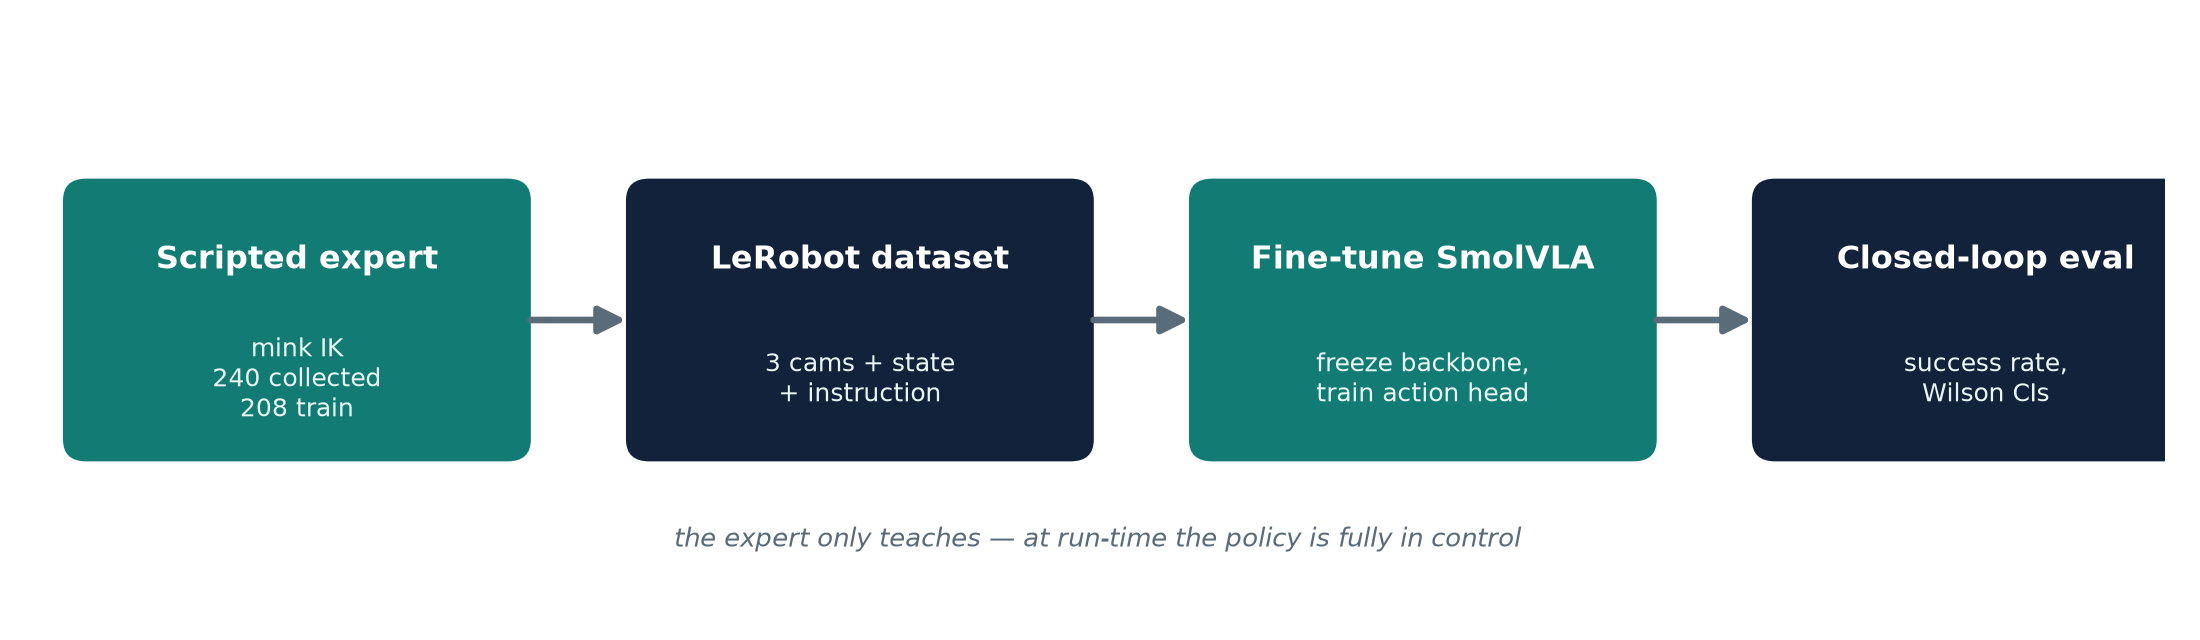
\includegraphics[width=\textwidth,
    alt={A four-stage pipeline: scripted expert with mink inverse kinematics generating 208 training demonstrations, a LeRobot dataset of three cameras plus state plus instruction, fine-tuning SmolVLA with a frozen backbone, and closed-loop evaluation with Wilson confidence intervals.}]{figures/fig_pipeline}
\end{center}
\caption{The experimental pipeline. A scripted inverse-kinematics expert generates
demonstrations, which are converted to the LeRobot dataset format and used to
fine-tune SmolVLA (backbone frozen, action expert trained); the policy is then
evaluated closed-loop.}
\label{fig:pipeline}
\end{figure}

\section{Research design}
\label{sec:m-design}

\subsection{Research strategy}
\label{sec:m-strategy}
The work is an \emph{empirical, quantitative} study in the hypothetico-deductive mode:
each research question of \refsec{sec:rqs} becomes a prediction a controlled experiment
can confirm or refute, run at a sample size chosen so the outcome is informative rather
than anecdotal. Evidence is numerical --- success rates over many closed-loop rollouts
with interval estimates --- supplemented by qualitative tracing where a number alone
does not identify a cause (\refsec{sec:results-diagnosis}).

It combines two activities usually kept apart: \emph{construction}, since no
off-the-shelf environment, expert or dataset existed; and \emph{controlled
experimentation} on the artefact so constructed. This is design-oriented engineering
research, in which an artefact is built to make a phenomenon observable and the
knowledge claim rests on what is measured. Artefact and findings therefore developed
together, and the build history is reported rather than tidied away
(\refsec{sec:m-dev}, \refsec{sec:results-journey}).

Because the artefact was built by the same person who evaluates it, the design separates
the two roles wherever it can: success is defined geometrically and scored by code, not
by inspection; the identical criterion gates collection and evaluation, so the
definition cannot drift; evaluation is automated end to end; and the deployment
checkpoint is chosen by a pre-declared rule. Where a claim rests on judgement, this is
stated.

\subsection{Why simulation}
\label{sec:m-whysim}
The entire study is conducted in the MuJoCo physics simulator
\parencite{todorov2012mujoco}. This is a methodological choice, not merely a
practical one, and it is justified on four grounds.

\begin{enumerate}
    \item \textbf{Statistical power.} The conclusions rest on more than 1{,}300
    closed-loop rollouts (\reftab{tab:experiments}) --- not attainable on hardware
    within an MSc project, but a few days of headless compute in simulation. Since
    \refsec{sec:bg-eval} identifies under-powered evaluation as the dominant hazard in
    this literature, a setting that makes adequate samples affordable answers it
    directly.
    \item \textbf{Ground truth.} The displacement experiment of
    \refsec{sec:results-lookup} needs the exact pose of every object and of the gripper
    at closure, and objects placed at prescribed positions repeatably to the
    millimetre --- free in simulation, and requiring motion capture on hardware.
    \item \textbf{Control of confounds.} Testing whether a policy localises the named
    item or recalls its position requires holding everything constant except object
    position, including the random seed.
    \item \textbf{Cost and safety.} No hardware was available under the project's
    budget, and a \SI{1.3}{m}-reach industrial arm running an unvalidated learned
    policy would require a safety case disproportionate to the question asked.
\end{enumerate}

The limitation is stated plainly: no claim of sim-to-real transfer is made, no domain
randomisation is employed, and the reality gap of \refsec{sec:bg-sim} applies in full.
To keep a later transfer study possible, the pipeline uses tooling a real-robot study
would also use --- LeRobot \parencite{cadene2024lerobot} and manufacturer-derived models
of a real arm, gripper and base.

\subsection{Phased structure of the study}
\label{sec:m-phases}
The research proceeded in three phases (\reftab{tab:phases-study}). Each ended in an
empirical result that determined the next, and they are reported in that order in
\refChap{chap:results} rather than as a single pre-planned design, because the
reasoning from one to the next is part of the contribution.

\begin{table}[ht]
\caption{The three phases of the study. Each phase terminated in a result that
determined the scope of the next.}
\begin{center}
\tagpdfsetup{table/header-rows={1}}
\begin{tabular}{p{0.13\textwidth}p{0.24\textwidth}p{0.24\textwidth}p{0.27\textwidth}}
\toprule
Phase & Setting & Question & Outcome that set the next phase \\
\midrule
1. Benchmark feasibility &
RoboCasa kitchen benchmark, Franka on a mobile base &
Can deployable small models perform an established benchmark after task-specific
fine-tuning? &
No: 0/20 for both SmolVLA and ACT. Difficulty had to be reduced along every axis at
once. \\
\addlinespace
2. Controlled pilot &
Fixed-base UR10e, single cube, five positions &
Can the same small models learn a controlled task, and what dominates performance? &
Yes ($\sim$47--53\%), but a metric bug, duplicated data and a memory ceiling
mattered more than model choice. \\
\addlinespace
3. Main study &
Simulated supermarket: UR10e on an Omron base, four grocery items, language-conditioned &
What can a compact VLA do under a \SI{12}{GB} ceiling, and what has it actually
learned? &
Reported in full in \refChap{chap:results}. \\
\bottomrule
\end{tabular}
\end{center}
\label{tab:phases-study}
\end{table}

The narrowing follows \refsec{sec:bg-sim}'s diagnosis of \emph{why} RoboCasa is hard
for a small model. Phase 2 removed all four compounding difficulties at once; Phase 3
reintroduced the task-relevant complexity while retaining experimental control. Phases 1
and 2 are reported in \refsec{sec:results-journey}; the remainder of this chapter
describes Phase 3.

\subsection{From research questions to experiments}
\label{sec:m-rq-map}
\reftab{tab:rqmap} maps each research question onto the experiments that answer it
and the measurement each yields. The catalogue of experiments itself, with sample
sizes and conditions, is given in \refsec{sec:m-experiments}.

\begin{table}[ht]
\caption{Mapping from research questions (\refsec{sec:rqs}) to experiments and
measurements. Experiment identifiers refer to \reftab{tab:experiments}.}
\begin{center}
\tagpdfsetup{table/header-rows={1}}
\begin{tabular}{p{0.09\textwidth}p{0.36\textwidth}p{0.11\textwidth}p{0.32\textwidth}}
\toprule
RQ & Prediction to be tested & Experiments & Measurement \\
\midrule
RQ1 & A compact VLA fine-tuned within \SI{12}{GB} completes the task more often than
not. & E3, E7 & Task-completion rate with Wilson interval; peak GPU memory. \\
\addlinespace
RQ2 & At this scale, changes to data, metrics and observability move performance more
than changes to model capacity. & E1, E2, E4, E8 & Success rate before and after each
intervention; same-task comparison against a policy $1/8$ the size. \\
\addlinespace
RQ3 & If the policy is language-conditioned, the reach follows the instruction; if it
is \emph{visually grounded}, the reach follows the object when the two are decoupled.
& E5, E6, E7 & Gripper lateral position at gripper closure versus actual and versus
trained item position. \\
\addlinespace
RQ4 & The failure is localisable to one stage of the
perception--language--grasp--place chain and correctable without adding capacity. &
E4, E6 & Per-stage outcome (grasp versus placement); success rate after each targeted
change. \\
\bottomrule
\end{tabular}
\end{center}
\label{tab:rqmap}
\end{table}

\section{Development methodology}
\label{sec:m-dev}
The artefact was developed \emph{iteratively and incrementally}: as a sequence of
small, independently runnable stages, each with its own verification, so a defect could
be attributed to a stage rather than to the system as a whole. This matters because the
thesis's central methodological claim --- that diagnosis outperforms scaling --- is
only actionable if failures can be localised.

\subsection{Increments and their acceptance criteria}
\label{sec:m-increments}
\reftab{tab:increments} lists the increments in order with the check that had to pass
before the next began. Every increment is verified against a criterion that does
\emph{not} depend on the learned policy, so when a policy later fails, the stages
beneath it are already validated.

\begin{table}[ht]
\caption{Development increments and the acceptance check applied to each before
proceeding. Each check is independent of the learned policy.}
\begin{center}
\tagpdfsetup{table/header-rows={1}}
\begin{tabular}{p{0.05\textwidth}p{0.30\textwidth}p{0.55\textwidth}}
\toprule
\# & Increment & Acceptance check \\
\midrule
1 & Scene model: base, arm, gripper, shelf, products, cameras &
Arm converges to commanded joint targets under gravity compensation; products rest
stably; all three cameras render headlessly through EGL. \\
\addlinespace
2 & Inverse-kinematics solver for grasp and place poses &
Solutions lie on the kinematic branch the position servos can track, seeded from the
home configuration; no joint wrapping beyond $\pm 2\pi$. \\
\addlinespace
3 & Scripted expert trajectory &
Per-item success under per-episode jitter measured over repeated runs
(\reftab{tab:grasptune}); items with unreliable expert performance excluded rather
than carried into the dataset. \\
\addlinespace
4 & Demonstration recorder and dataset conversion &
Every retained episode passes the \emph{same} geometric placement check later used to
score the policy; frame counts, camera streams, state/action dimensions and
instruction labels verified on the converted dataset. \\
\addlinespace
5 & Fine-tuning configuration &
Training completes within the \SI{12}{GB} budget with peak memory recorded; loss
decreases; checkpoints written at fixed intervals. \\
\addlinespace
6 & Closed-loop evaluation harness &
Scripted expert scored through the harness reproduces its known success rate,
confirming the harness measures what it claims to; normalisation statistics loaded
from the checkpoint under test. \\
\addlinespace
7 & Multi-item orchestrator &
Arm returns to the in-distribution home configuration between items; basket contents
persist across picks; retry logic disabled for measurement runs. \\
\bottomrule
\end{tabular}
\end{center}
\label{tab:increments}
\end{table}

\subsection{The diagnostic loop}
\label{sec:m-diagnostic-loop}
Where a trained policy underperformed, the response followed a fixed rule, adopted
after the Phase-2 experience described in \refsec{sec:results-journey}:

\begin{enumerate}
    \item \textbf{Reproduce and instrument} the failure over enough trials to
    establish that it is systematic rather than sampling noise.
    \item \textbf{Trace a single episode} frame by frame, recording object and
    gripper poses, to establish \emph{where} in the perception--language--grasp--place
    chain the behaviour departs from the demonstration.
    \item \textbf{Form a mechanism hypothesis} that predicts something not yet
    measured.
    \item \textbf{Change one thing} that the hypothesis implicates --- the data, the
    observation, or the environment --- and re-measure under the identical protocol.
    \item \textbf{Only then consider capacity.} Increasing model size, training
    steps or dataset volume was treated as the last resort, not the first.
\end{enumerate}

This rule produced the sequence in \refsec{sec:results-diagnosis}, and also the most
uncomfortable result in the thesis: applying step~3 to an apparently successful
grounding result predicted that displacing an item would not move the reach, and testing
that prediction (\refsec{sec:results-lookup}) overturned the stronger interpretation of
the earlier finding.

\subsection{Tooling, environment and reproducibility}
\label{sec:m-tooling}
Development used Python with MuJoCo~3.9, \texttt{mink} for differential inverse
kinematics \parencite{zakka2024mink}, and Hugging Face LeRobot for dataset format,
training and policy implementations \parencite{cadene2024lerobot}; assets are the
robosuite grocery and Omron meshes \parencite{zhu2020robosuite} and the UR10e and
Robotiq models from the MuJoCo Menagerie \parencite{deepmind2022menagerie}. All
training and evaluation ran on a single NVIDIA RTX~A2000 with \SI{12}{GB} of VRAM ---
the constraint the thesis is organised around, not an incidental fact about the machine.

Three measures support reproducibility: the pipeline is decomposed into single-purpose
scripts runnable in isolation (Appendix~\ref{app:Implementation}); library versions are
pinned; and the seed, hyper-parameters, success criteria and scene constants are
reported exactly. Source is version-controlled so a checkpoint can be matched to the
code that produced it.

\section{Simulated supermarket environment}
\label{sec:m-env}
The environment is constructed programmatically as a single MuJoCo~3.9 model
\parencite{todorov2012mujoco}, rendered off-screen through EGL for headless data
generation. The mobile manipulator comprises an Omron LD-60 mobile base
(robosuite mesh, \parencite{zhu2020robosuite}), a UR10e six-degree-of-freedom arm and a
Robotiq 2F-85 two-finger gripper (MuJoCo Menagerie,
\parencite{deepmind2022menagerie}). The arm is re-parented onto the base's
support column at a height of approximately \SI{0.70}{m}; without intervention the
arm's position servos droop by several centimetres under gravity, so
\emph{gravity compensation} is enabled on the arm subtree
(\texttt{body\_gravcomp}) so that the servos reach commanded configurations
accurately. The model exposes ten actuators: six position servos for the arm
joints, one for the gripper, and three velocity servos for the base
(forward, lateral and yaw). During each pick the base is held stationary by its
velocity servos; language-guided navigation is deferred to future work
(\refsec{sec:future}). To permit precise parking, the mobile-joint friction-loss
was reduced from the mesh default of 250 to 15.

Several physics settings required tuning to obtain stable, realistic behaviour.
Gravity compensation on the arm subtree is essential: without it the position servos
settle several centimetres below their commanded configuration under the arm's own
weight, which both misaligns the grasp and breaks the correspondence between the
recorded action (the commanded target) and the achieved pose. Grip stability is the
other principal concern. The robosuite grocery meshes are smooth and the parallel
gripper is rigid, so a friction-only grasp is marginal during the accelerations of
transport; increasing the product friction coefficient and enabling additional
no-slip solver iterations while the item is held keeps it secure, while disabling those
iterations at release lets it fall freely rather than being flung. Contact softness is
set so that grasps are compliant enough not to eject the item on contact yet stiff
enough to hold it. These values were established empirically against the scripted
expert's success rate, and they matter for learning as much as for the expert:
demonstrations generated under unstable physics would teach the policy to reproduce
unstable behaviour.

Products are textured grocery meshes from robosuite \parencite{zhu2020robosuite} --- a milk carton, cola can,
bread loaf, cereal box and water bottle --- selected over primitive shapes for
visual realism so that the pretrained perception of the VLA has meaningful cues to
exploit. The assembled workspace is shown in \reffig{fig:system}, and the
task-relevant geometry is given as a top-down schematic in
\reffig{fig:layout}. The five products rest along the shelf front at lateral
positions $y \in \{-0.26, -0.13, 0.00, 0.15, 0.34\}$\,\si{m}; these were chosen to
lie within the arm's reliable grasp zone so that per-episode jitter never forces
an item into a marginal, extended-reach configuration. The basket is mounted on
the base deck at approximately $(x,y)=(0.24, 0.00)$\,\si{m}.

\begin{figure}[ht]
\begin{center}
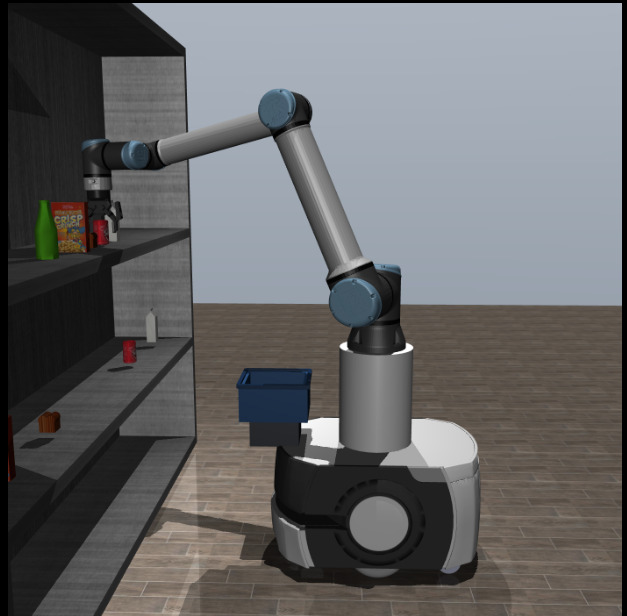
\includegraphics[width=0.75\textwidth,
    alt={The simulated mobile manipulator: an Omron mobile base with a UR10e arm and gripper, facing a stocked supermarket shelf, with a basket mounted on the base.}]{figures/image.jpeg}
\end{center}
\caption{The simulated supermarket workspace: an Omron mobile base carrying a
UR10e arm and Robotiq gripper, a stocked shelf of textured grocery meshes, and an
onboard basket as the drop target.}
\label{fig:system}
\end{figure}

\begin{figure}[ht]
\begin{center}
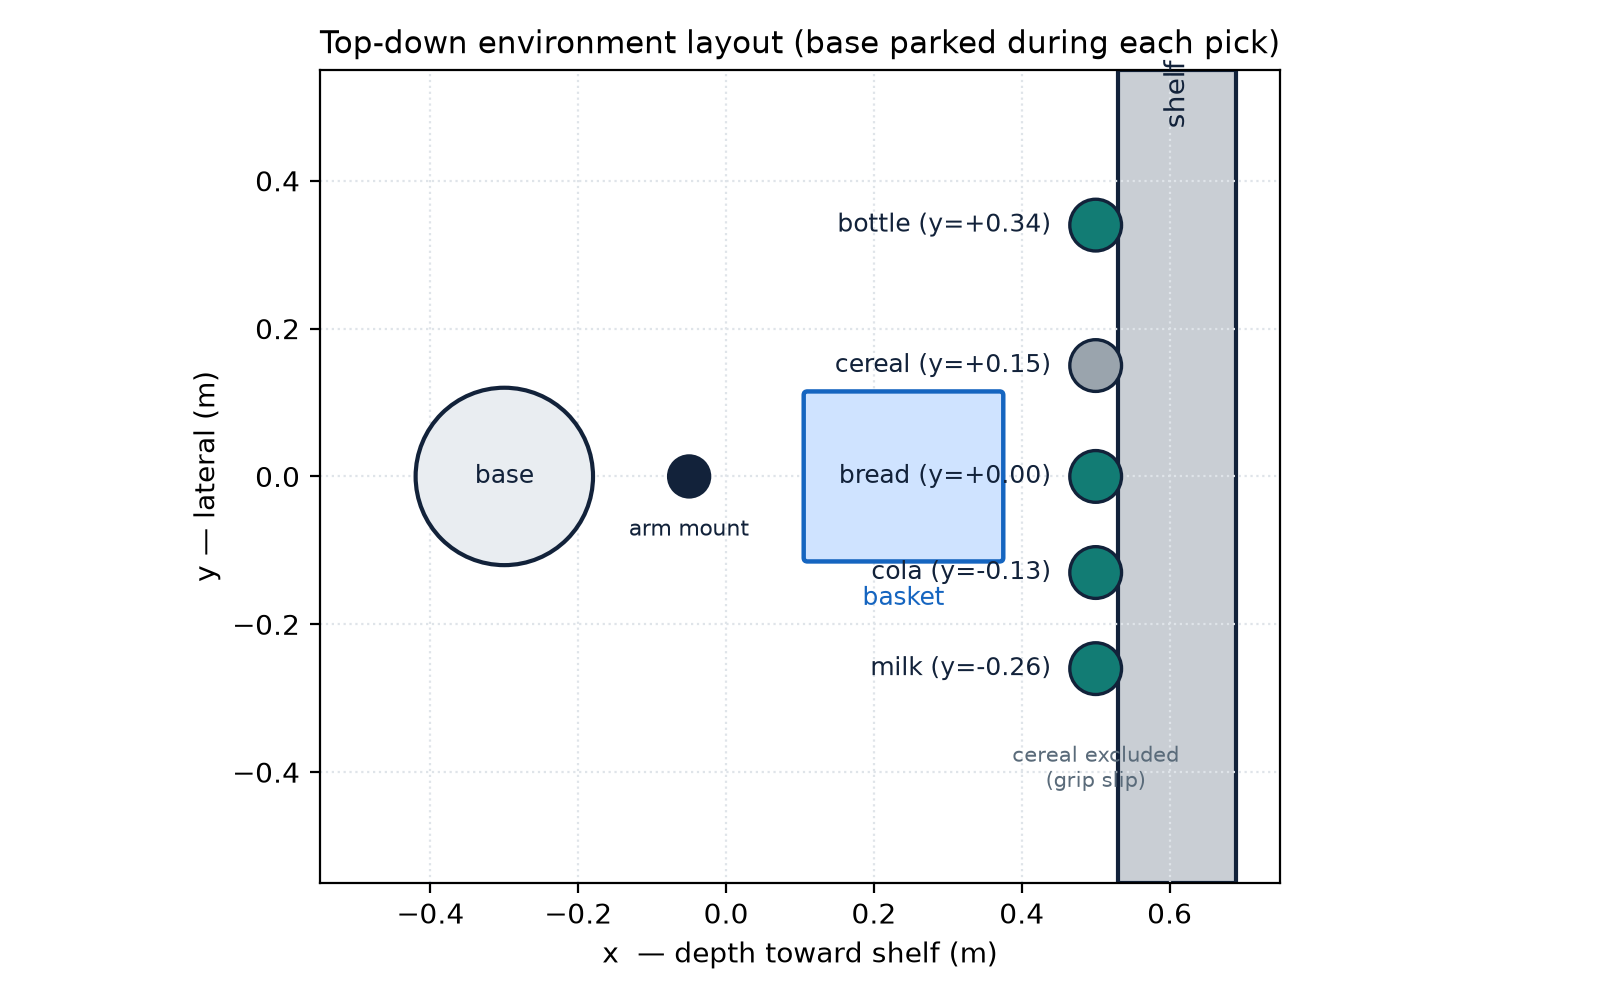
\includegraphics[width=0.85\textwidth,
    alt={A top-down schematic of the environment showing the parked base, the arm mount, the basket on the deck, and the five grocery items along the shelf front at their lateral positions.}]{figures/fig_env_layout}
\end{center}
\caption{Top-down schematic of the task geometry (metres, base frame). Products
rest along the shelf front at the indicated lateral positions, all at $x=0.880$; the
cereal box is shown for completeness but is excluded from training and from all
reported results, as it slips in the two-finger gripper. Note that the water bottle
($y=+0.34$), not the milk carton ($y=-0.26$), is the most laterally displaced item.}
\label{fig:layout}
\end{figure}

\subsection{Arm, gripper and workspace}
\label{sec:m-arm}
The UR10e is a six-degree-of-freedom serial manipulator with a nominal reach of
approximately \SI{1.3}{m} and a spherical wrist, which gives a large, dexterous
workspace well suited to reaching across a shelf and over the basket. The six
revolute joints are driven by MuJoCo position servos; commanding a joint
configuration and stepping the physics under gravity compensation causes the arm to
converge to that configuration. Because the arm is redundant for a purely positional
grasp target only in orientation (six joints for a six-dimensional pose), the
inverse-kinematics problem is well posed but sensitive to the branch of the solution,
which motivates the home-seeding described in \refsec{sec:m-ik}.

The Robotiq 2F-85 is an under-actuated parallel gripper with an \SI{85}{mm} stroke,
modelled with the tendon-driven finger coupling from the MuJoCo Menagerie. Its single
control input is mapped to a normalised opening in $[0,1]$, which is the seventh
dimension of both the state and the action. Because the fingers are rigid and the
robosuite meshes are smooth, a friction-only grip is prone to slipping during the
accelerations of transport; this is countered by enabling additional no-slip solver
iterations while the item is held and by keeping transport motions gentle, and the
no-slip iterations are disabled at the instant of release so the item falls freely
into the tote rather than being flung.

The policy observes the scene through three cameras, illustrated in
\reffig{fig:cameras}: a \emph{wrist} camera (eye-in-hand, \SI{75}{\degree} field of
view) for the close-up grasp; a \emph{scene} camera facing the shelf for object
localisation; and a \emph{basket} camera aimed at the drop target. The basket camera
was not part of the original design: it was added in response to the failure analysis
of \refsec{sec:results-diagnosis}, where poor observability of the drop target was
identified as a cause of the initial placement failures. It is described here with the
rest of the final configuration for coherence. Each camera is rendered at
$96\times96$ pixels. These three images, together with the arm's
seven-dimensional proprioceptive state and the text instruction, constitute the
entire input to the policy; crucially, \emph{no object coordinates or segmentation
are provided}, so any localisation of the named item must be derived from pixels. It
should be noted at the outset --- and is established in \refsec{sec:results-lookup} ---
that withholding object coordinates does not by itself compel the policy to localise:
because each item occupies a fixed position throughout the demonstrations, associating
the item word with a memorised trajectory also fits the data, and that is what the
trained policy is found to do.

\begin{figure}[ht]
\begin{center}
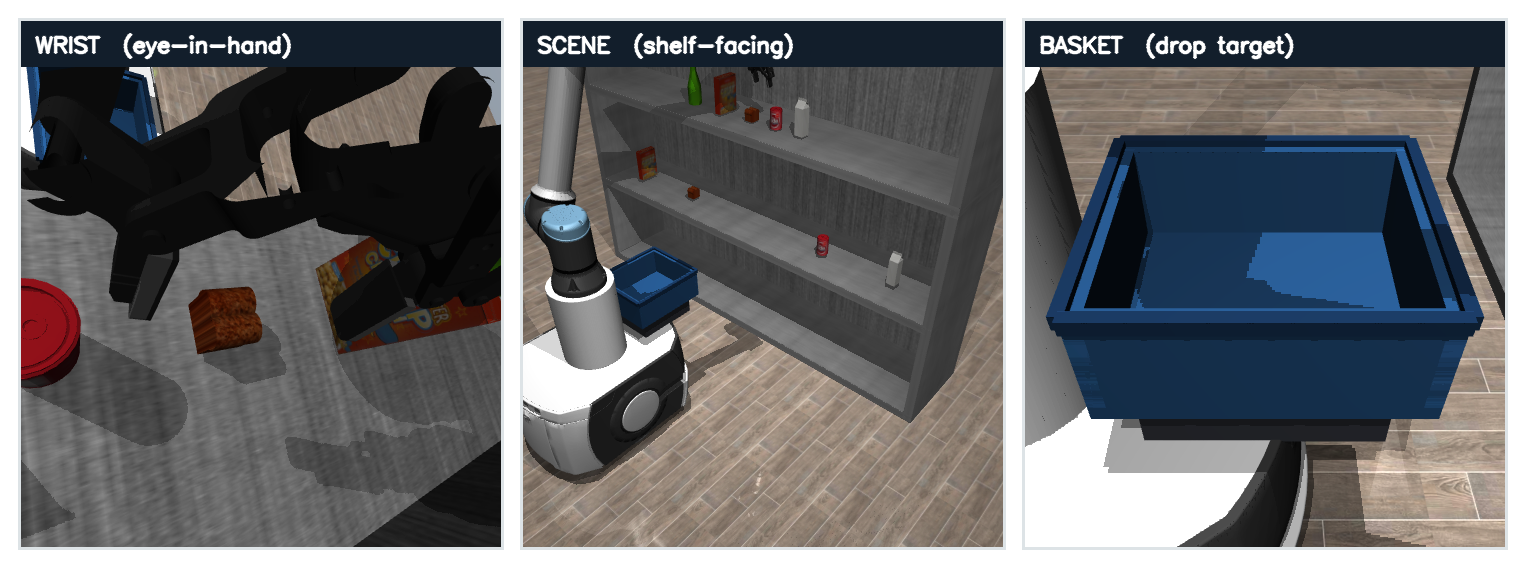
\includegraphics[width=\textwidth,
    alt={Three camera views: a wrist eye-in-hand view of the gripper, a scene view of the shelf, and a basket view of the drop target.}]{figures/camera_views}
\end{center}
\caption{The three synchronised camera views the policy receives every step:
wrist (eye-in-hand), scene (shelf-facing) and basket (drop target).}
\label{fig:cameras}
\end{figure}

\subsection{Rendering and image preprocessing}
\label{sec:m-render}
Camera frames are produced by MuJoCo's off-screen renderer through EGL, which allows
data generation and evaluation to run without a display --- essential for headless,
scripted collection of hundreds of episodes. Each camera renders an RGB image that is
resized to $96\times96$ before being passed to the policy. This modest resolution is a
deliberate compromise: it is large enough to localise the products and read the drop
target, but small enough that three streams can be encoded by the backbone within the
memory budget and at an interactive rate. At both training and inference the images
pass through the policy's pre-processor, which normalises pixel values and arranges the
channels as the backbone expects; the same pre-processor is used in both phases, so the
policy never sees an image distribution at test time that differs from training. The
live interactive viewer used for qualitative inspection renders through a display
rather than EGL and is used only for visualisation, not for measured results.

\section{Scripted expert and inverse kinematics}
\label{sec:m-expert}

\subsection{Differential inverse kinematics}
\label{sec:m-ik}
Grasp and place poses are solved with \texttt{mink} \parencite{zakka2024mink}, a
MuJoCo-native differential inverse-kinematics library. At each solver iteration the joint velocity
$\dot{\mathbf{q}}$ is obtained by solving a small quadratic program that minimises
the weighted end-effector task error subject to kinematic limits,
\begin{equation}
\min_{\dot{\mathbf{q}}}\;
\sum_{k} \big\lVert \mathbf{J}_k \dot{\mathbf{q}} - \mathbf{v}_k^{\star} \big\rVert^2
\quad\text{s.t.}\quad
\dot{\mathbf{q}}_{\min} \le \dot{\mathbf{q}} \le \dot{\mathbf{q}}_{\max},
\label{eq:ik}
\end{equation}
where $\mathbf{J}_k$ is the task Jacobian and $\mathbf{v}_k^\star$ the desired task
velocity for task $k$ (end-effector position and orientation). The mobile base is
pinned by a velocity limit and the arm respects a configuration limit, so only the
six arm joints move. Because \eqref{eq:ik} is solved iteratively from the current
configuration, it is a \emph{local} solver: grasp IK is therefore seeded from the
arm's actual home configuration, which yields a solution on the same kinematic
branch that the position servos can subsequently track. Seeding from an arbitrary
pose was found to produce joint solutions that wrap beyond $\pm 2\pi$ or that the
servo cannot follow, causing the gripper to close off-centre.

\subsection{Pick-and-place trajectory}
\label{sec:m-traj}
Because the target shelf bay is boxed in from above, the item cannot simply be
lifted vertically clear of the shelf. Instead the expert executes a top-down grasp
followed by a \emph{frontal extraction}: the grasped item is pulled straight out of
the shelf front at grasp height before being carried to the basket. The full phase
sequence is listed in \reftab{tab:phases}. Grip stability on the smooth robosuite
meshes is maintained by enabling no-slip solver iterations during transport; these
are disabled immediately before release so the item drops cleanly into the tote.

\begin{table}[ht]
\caption{Phases of the scripted pick-and-place trajectory. Interpolation steps are
executed under the arm position servos, stepping the physics between waypoints.}
\begin{center}
\tagpdfsetup{table/header-rows={1}}
\begin{tabular}{lll}
\toprule
Phase & Gripper & Purpose \\
\midrule
Home              & open          & settle at the trained start pose \\
Pre-grasp         & open          & position above the item \\
Grasp             & open          & descend to grasp height \\
Close             & open$\to$closed & secure the item \\
Lift              & closed        & raise into the opened shelf bay \\
Extract           & closed        & pull straight out of the shelf front \\
Approach          & closed        & move over the basket \\
Lower / place     & closed        & descend over the tote \\
Release           & closed$\to$open & drop the item (no-slip disabled) \\
Settle            & open          & hold while the item settles \\
\bottomrule
\end{tabular}
\end{center}
\label{tab:phases}
\end{table}

\subsection{Per-item grasp tuning}
\label{sec:m-grasp}
Reliable grasping required per-item parameters, summarised in
\reftab{tab:grasptune}: the finger-closing yaw, the grip height (wrist-to-item
offset) and the item's rest position. The cereal box, being the widest item,
requires the fingers to close across its narrow face; the water bottle, being
tall, requires a higher grip point for a stable hold; and the milk carton was
moved inward from the reach edge to prevent it toppling under jitter. With these
tunings the expert succeeds, under per-episode jitter, on the four retained items
with rates of 100\% (cola), 100\% (bread), 98\% (milk) and 96\% (bottle). The
cereal box is excluded from training: even with a $90^\circ$ grasp yaw it slips in
transport, and reliably teaching a policy from unreliable demonstrations is not
possible.

\begin{table}[ht]
\caption{Per-item grasp parameters and scripted-expert success rate (with
per-episode positional jitter).}
\begin{center}
\tagpdfsetup{table/header-rows={1}}
\begin{tabular}{lccc}
\toprule
Item & Grasp yaw & Notable tuning & Expert success \\
\midrule
Cola can     & default & ---                         & 100\% \\
Bread loaf   & default & ---                         & 100\% \\
Milk carton  & default & moved inward from reach edge & 98\% \\
Water bottle & default & higher grip point           & 96\% \\
Cereal box   & $90^\circ$ & \emph{excluded} (grip slip) & --- \\
\bottomrule
\end{tabular}
\end{center}
\label{tab:grasptune}
\end{table}

\section{Demonstration collection and dataset}
\label{sec:m-data}
For each successful episode, the recorder stores, per control step: the three
camera images ($96\times96$), the seven-dimensional state (six arm joint angles and
the gripper opening), the seven-dimensional action (the executed servo command),
and a natural-language instruction. To make the policy \emph{language-conditioned}
rather than reliant on a single memorised sentence, the instruction is drawn from a
set of six paraphrase templates (for example, ``pick up the
\{item\} and place it in the basket'', ``grab the \{item\} and put it in the
basket''), with one template sampled per episode. The identical template module is
used at inference to guarantee train--deploy consistency. Each item's planar
position is randomly jittered by up to \SI{2.5}{cm} per episode, and the grasp IK is
re-solved on the settled position so that the demonstrations cover a distribution
of grasp poses rather than a single canonical trajectory.

Only \emph{successful} demonstrations are retained. Success is verified physically at
the end of each scripted episode by checking that the target item has come to rest
inside the basket footprint and low (not perched on the rim), using the same
geometric criterion later applied to the learned policy; episodes that fail this check
are discarded rather than saved. This guards against a subtle failure mode observed in
the pilot study, where an over-permissive success check admitted demonstrations in
which the item was merely near the basket, teaching the policy an imprecise notion of
``placed''. Verifying demonstrations with the same metric used for evaluation keeps
the definition of success consistent across data collection, training and testing.

A design choice that proved decisive concerns the \emph{episode boundary}:
demonstrations end at the instant of placement. The return-to-home motion is a
reset for the next episode rather than part of the demonstration, and recording it
in an earlier iteration taught the policy to move away immediately after releasing,
knocking the item back out of the basket (\refsec{sec:results-diagnosis}).

In total, 240 successful demonstrations were collected (60 per item across the four
retained items) and converted to the LeRobot dataset format (parquet plus encoded
video) \parencite{cadene2024lerobot}. Of these, \textbf{208 were used for training and 32
(8 per item) held out for validation}; all results reported in \refChap{chap:results}
therefore rest on 208 training demonstrations. The \SI{100}{Hz} recordings are subsampled by a
factor of five to \SI{20}{fps}, so that a fixed-length action chunk spans a useful
temporal horizon rather than a fraction of a second, and a per-item hold-out is
reserved for validation. Normalisation statistics are computed on the training
split and, critically, are frozen with the checkpoint (\refsec{sec:m-eval}).
\reffig{fig:dataset} shows a sample of the recorded streams.

\begin{figure}[ht]
\begin{center}
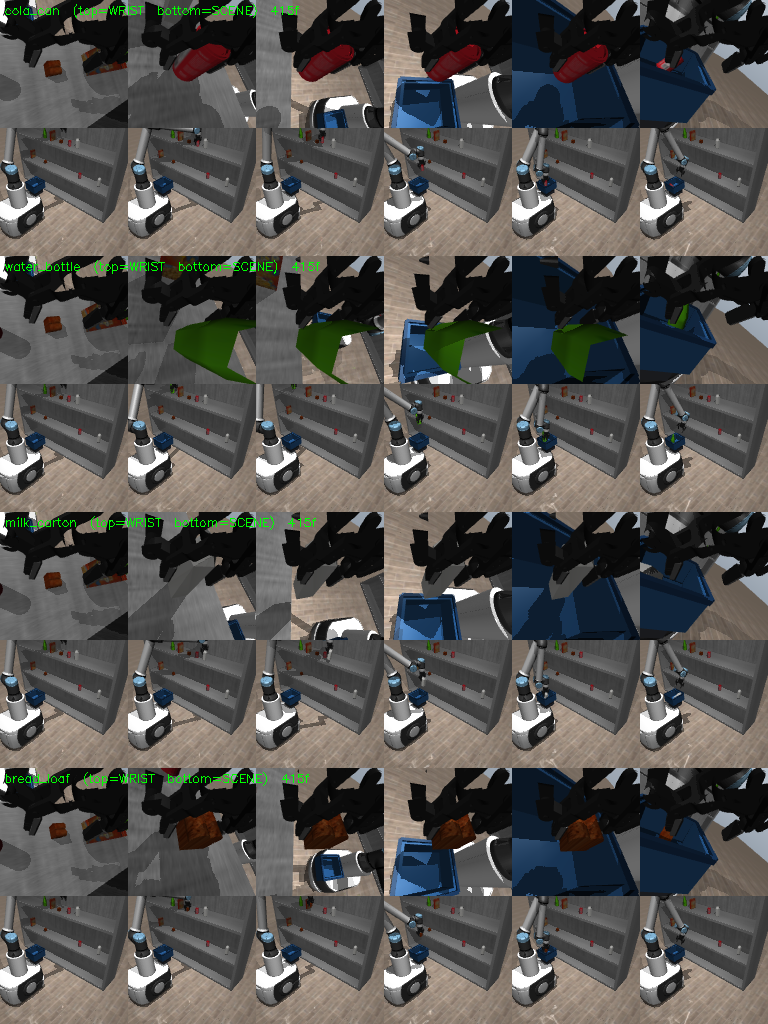
\includegraphics[width=\textwidth,
    alt={A filmstrip of recorded demonstration frames showing the wrist and scene camera streams across a pick-and-place for each item.}]{figures/dataset_preview}
\end{center}
\caption{A sample of the demonstration dataset: wrist and scene camera streams
across a pick-and-place, for each of the four training items. This sample predates
the addition of the basket camera (\refsec{sec:results-diagnosis}); the deployed
configuration records three streams per step.}
\label{fig:dataset}
\end{figure}

\reffig{fig:pickplace} shows key frames of the scripted trajectory that generates
these demonstrations.

\begin{figure}[ht]
\begin{center}
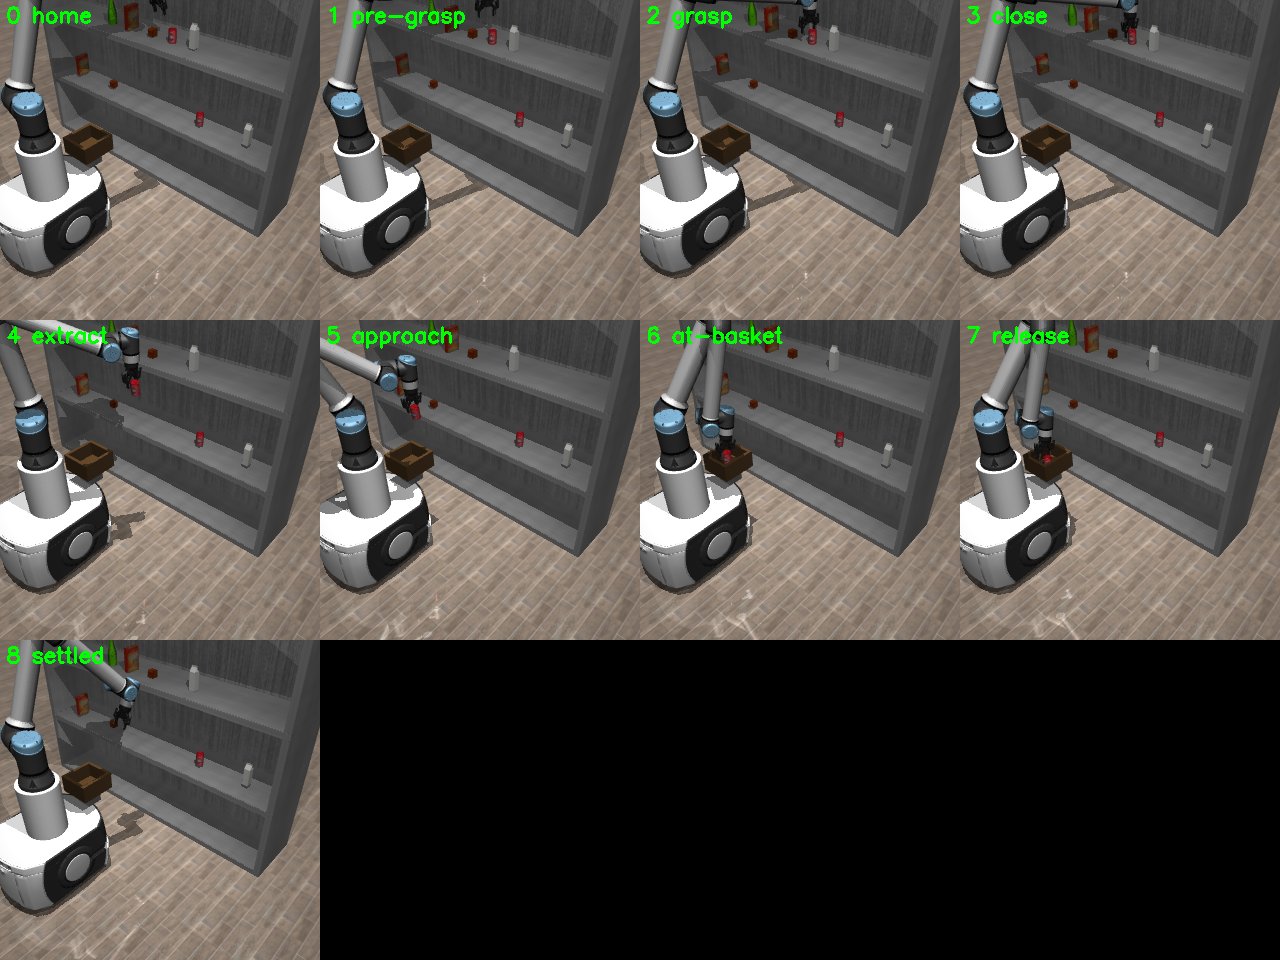
\includegraphics[width=\textwidth,
    alt={A filmstrip of the scripted pick-and-place: home, pre-grasp, grasp, lift, extract, carry over the basket, and place.}]{figures/pickplace_cola_can}
\end{center}
\caption{Key frames of the scripted-expert pick-and-place used to generate
demonstrations, from home pose through grasp, extraction and placement.}
\label{fig:pickplace}
\end{figure}

\subsection{Instruction generation and language conditioning}
\label{sec:m-lang}
Each demonstration is labelled with a natural-language instruction sampled, at
collection time, from a small library of paraphrase templates parameterised by the
item name --- for example ``pick up the \{item\}\ and place it in the basket'', ``grab
the \{item\}\ and put it in the basket'', ``take the \{item\}\ and drop it in the
basket''. Six templates across the four retained items yield 24 distinct
instructions in total (the full list is given in Appendix~\ref{app:Implementation}). The
purpose of this variety is to prevent the policy from binding to one exact sentence:
if every ``milk'' episode used identical wording, the model could in principle key on
the surface form rather than on the meaning. Paraphrasing forces the language signal
that survives across templates --- the item identity --- to be the informative one,
which is what a pretrained vision--language backbone is well placed to extract. The
identical template module is imported by both the data-collection and the inference
code, so the distribution of instructions seen at test time matches that seen during
training; this train--deploy consistency is a small but important guard against an
accidental mismatch that would degrade grounding. At inference the instruction is
tokenised and passed to the backbone alongside the images, exactly as during training.

\subsection{Observation and action spaces and the control loop}
\label{sec:m-spaces}
The observation supplied to the policy at each decision is the tuple
$(\mathbf{I}_{\text{wrist}}, \mathbf{I}_{\text{scene}}, \mathbf{I}_{\text{basket}},
\mathbf{s}, \ell)$, where each image $\mathbf{I}$ is a $96\times96$ RGB frame,
$\mathbf{s}\in\mathbb{R}^{7}$ is the proprioceptive state (six arm joint angles and
the gripper opening, the latter normalised to $[0,1]$), and $\ell$ is the tokenised
language instruction. The action $\mathbf{a}\in\mathbb{R}^{7}$ comprises six
absolute arm-joint targets and a gripper command in $[0,1]$; the policy predicts a
chunk of fifty such actions per forward pass.

The closed-loop control cycle proceeds as follows. The current observation is
assembled and passed through the pre-processor (which applies the frozen
normalisation statistics); the policy predicts a fifty-step action chunk; the chunk
is de-normalised by the post-processor; and its actions are applied to the arm
position servos and the gripper actuator, with the physics stepped exactly
twenty-five substeps per action (approximately \SI{20}{Hz}) before the next action.
When the chunk is exhausted the policy re-plans from the new observation. This
matches the horizon at which the demonstrations were sub-sampled, so that the action
chunk the policy learns to produce spans a comparable slice of real time. Between
consecutive items in a multi-item episode the arm is returned to its home
configuration (the same start state as during data collection) so that each pick
begins in-distribution; the scene itself is not reset, so previously collected items
remain in the basket.

\section{Fine-tuning SmolVLA}
\label{sec:m-train}
The policy is fine-tuned from the pretrained \texttt{smolvla\_base} checkpoint. The
architecture and the training split are summarised in \reffig{fig:architecture}.
SmolVLA couples a compact vision--language backbone (SmolVLM-2) with a
flow-matching action expert that predicts a chunk of future actions
\parencite{shukor2025smolvla, kiviranta2025smolvla}. The backbone tokenises the three
images and the instruction and, through interleaved cross- and self-attention,
produces a fused representation; SmolVLA additionally reduces the number of visual
tokens and lets the action expert read features from an intermediate backbone layer,
both of which lower inference cost \parencite{shukor2025smolvla}.

The action expert is trained by a \emph{conditional flow-matching} objective. Let
$\mathbf{a}_1$ denote a demonstrated action chunk and $\mathbf{a}_0\sim\mathcal{N}
(\mathbf{0},\mathbf{I})$ a noise sample; along the linear path
$\mathbf{a}_\tau=(1-\tau)\mathbf{a}_0+\tau\mathbf{a}_1$ for $\tau\in[0,1]$ the target
velocity is $\mathbf{a}_1-\mathbf{a}_0$. The network $v_\theta$ regresses this
velocity conditioned on the backbone features $\mathbf{c}$ and the proprioceptive
state,
\begin{equation}
\mathcal{L}(\theta)=\mathbb{E}_{\tau,\mathbf{a}_0,\mathbf{a}_1}
\big\lVert v_\theta(\mathbf{a}_\tau,\tau,\mathbf{c})-(\mathbf{a}_1-\mathbf{a}_0)\big\rVert^2 .
\label{eq:flow}
\end{equation}
At inference the learned field is integrated from a noise sample over a small number
of steps to produce an action chunk. Two properties of \eqref{eq:flow} matter here:
actions are continuous, which suits smooth manipulation; and sampling is
\emph{stochastic}, so repeated queries on the same observation give slightly
different chunks --- which is why success is a distribution to be estimated over many
trials rather than a fixed value (\refsec{sec:m-stats}).

\begin{figure}[ht]
\begin{center}
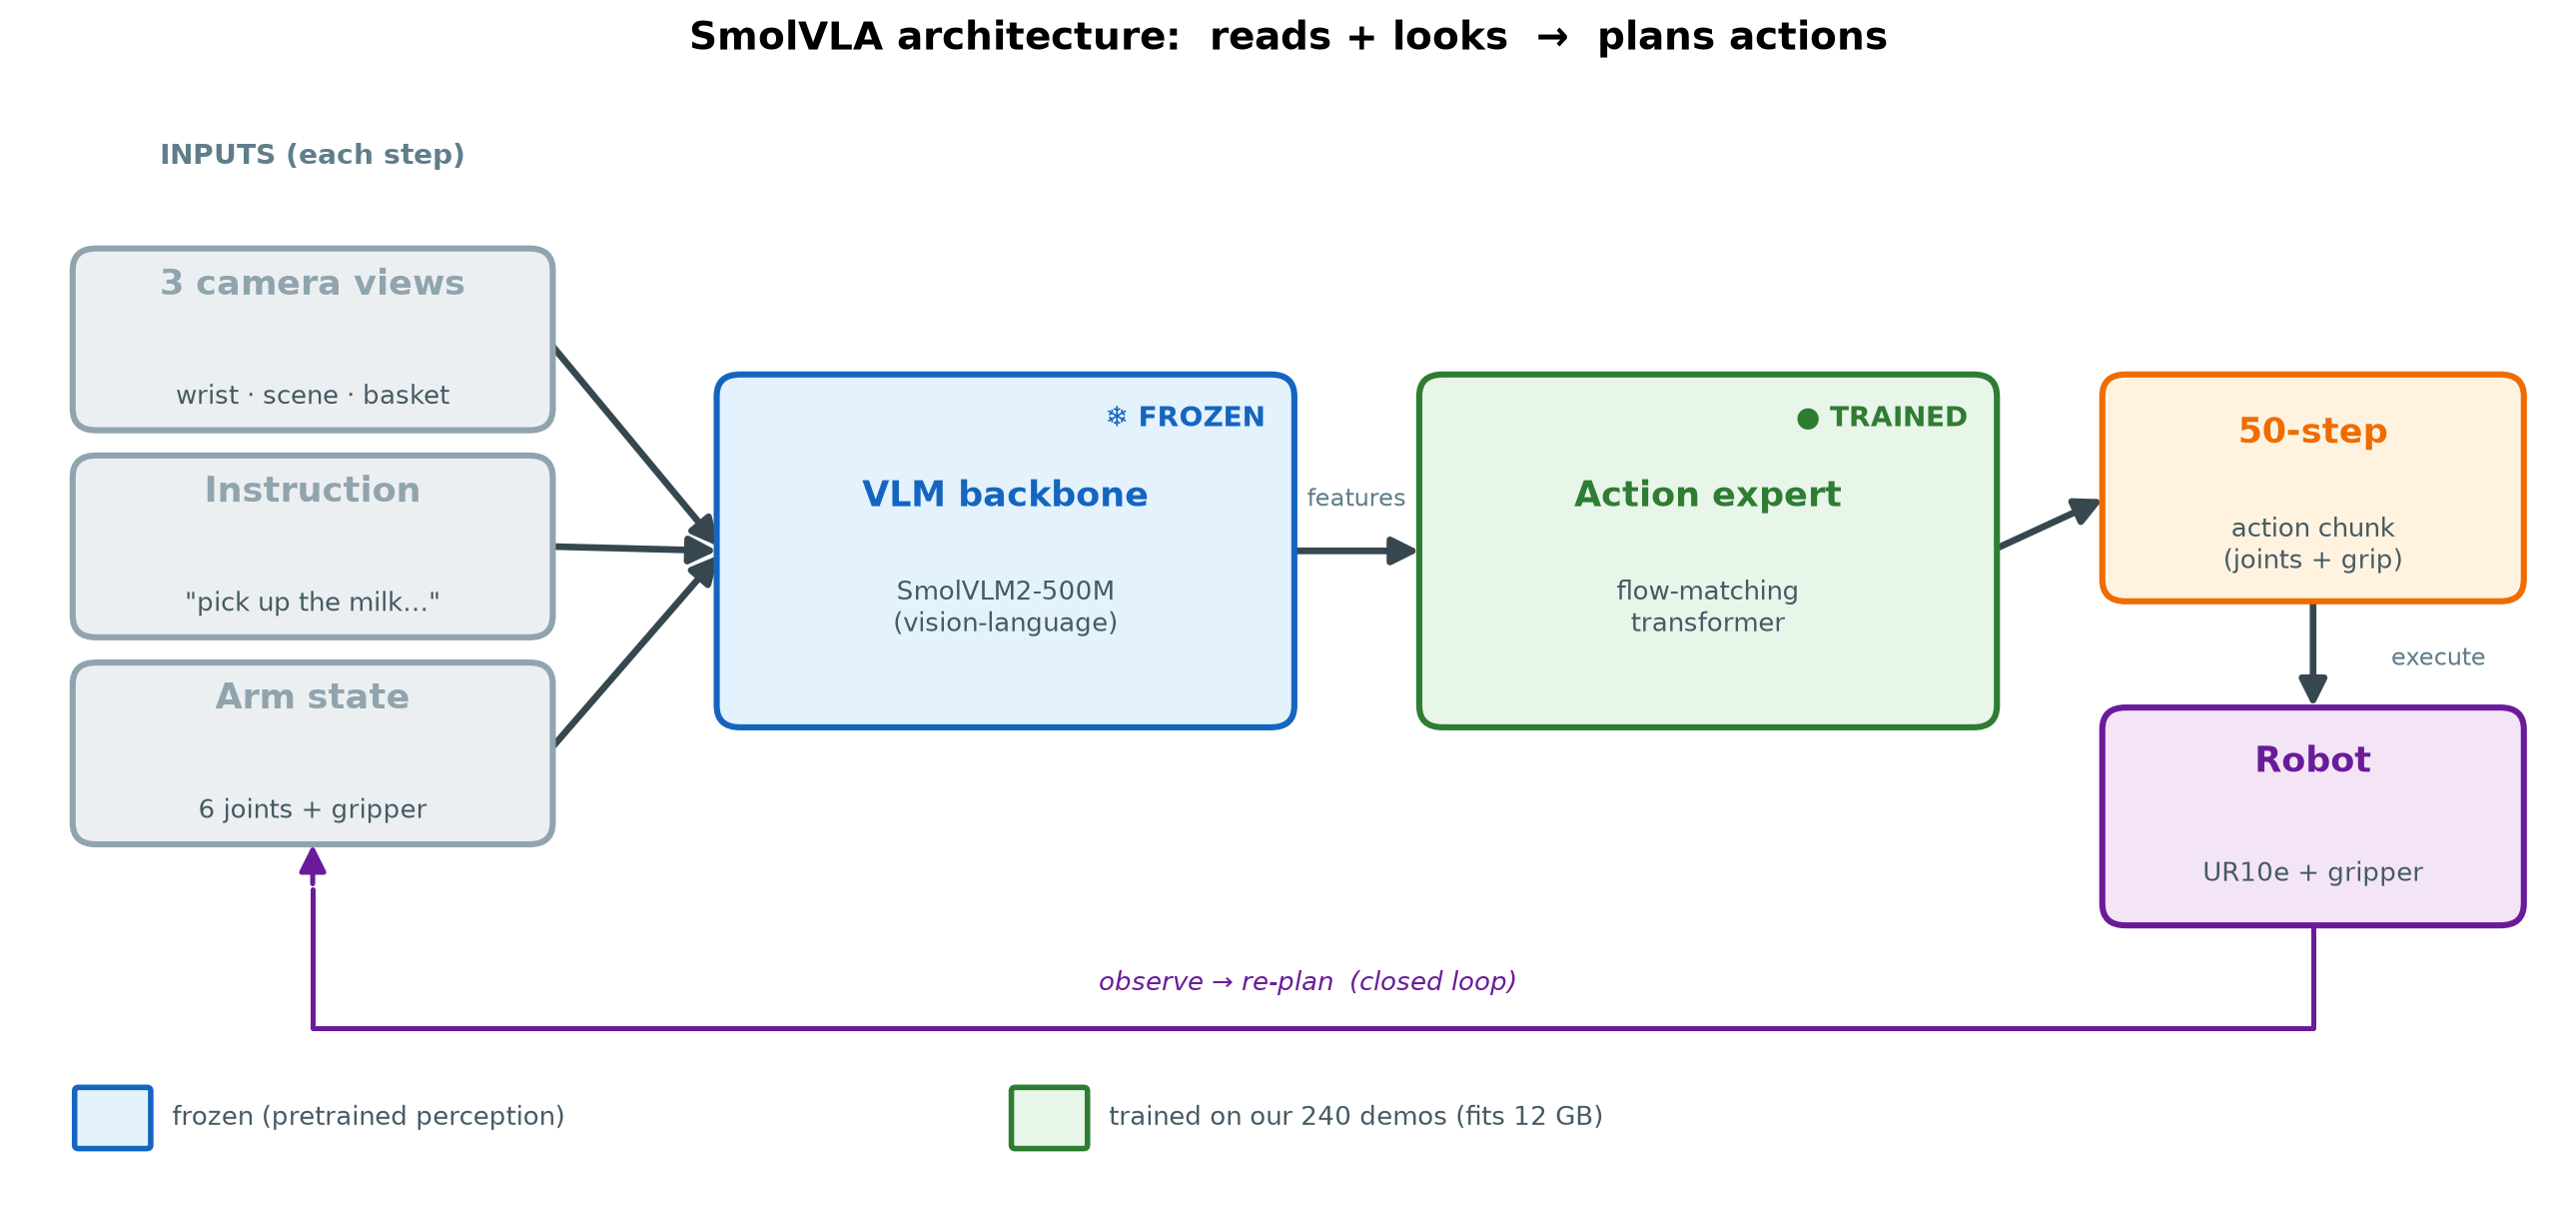
\includegraphics[width=\textwidth,
    alt={A block diagram of SmolVLA: three camera images, the instruction and the arm state feed a frozen vision-language backbone, whose features feed a trained flow-matching action expert that outputs a 50-step action chunk to the robot, in a closed loop.}]{figures/smolvla_architecture}
\end{center}
\caption{SmolVLA architecture and the training split used here. The pretrained
vision--language backbone (frozen) encodes the images and instruction; the action
expert (trained) maps its features and the arm state to a 50-step action chunk,
which is executed before re-planning.}
\label{fig:architecture}
\end{figure}

The decision that makes training feasible within \SI{12}{GB} is to \emph{freeze the
vision--language backbone} and train only the action expert. The rationale is
twofold. First, the backbone was pretrained on large image--text and robot corpora
and already provides strong perception and language grounding; back-propagating
into its roughly 400~million parameters from only 208 training demonstrations would risk
overfitting and catastrophic forgetting of that prior
\parencite{xiang2026posttraining, kiviranta2025smolvla}. In effect, the model already
knows what the objects are and what the words mean, so fine-tuning need only learn
the motor mapping for this specific embodiment. Second, freezing avoids storing
activations for a backward pass through the backbone: the frozen configuration
trains in approximately \SI{3}{GB}, whereas even partially unfreezing the vision
encoder alongside three camera streams exceeded the budget in the preliminary study
(\refsec{sec:results-journey}).

Training uses a batch size of eight for 20{,}000 optimisation steps: each step
draws eight (observation, action-chunk) samples, computes the flow-matching loss,
averages the gradient over the eight, and applies one update. Averaging over a
mini-batch reduces gradient variance relative to a single sample while remaining
within memory; eight was the largest batch that fit comfortably. Training takes
approximately four hours on an NVIDIA RTX~A2000 (\SI{12}{GB}). A checkpoint is
saved every 5{,}000 steps, yielding four candidate snapshots (5k, 10k, 15k and 20k
steps) for the selection procedure below. Complete hyper-parameters are listed in
Appendix~\ref{app:Implementation}.

\section{Experimental design}
\label{sec:m-experiments}
The preceding sections describe how the artefact is built; this one specifies what is
done with it. The measurement procedure itself follows in \refsec{sec:m-eval}.

\subsection{Variables}
\label{sec:m-variables}
Across the experiments, the following are \emph{manipulated} one at a time:

\begin{itemize}
    \item \textbf{Policy architecture} --- SmolVLA (450\,M, language-conditioned)
    versus ACT (52\,M, no language input), trained on identical data (E8).
    \item \textbf{Training checkpoint} --- the four snapshots at 5k, 10k, 15k and
    20k optimisation steps (E3).
    \item \textbf{Instruction} --- which item the text names, with the scene held
    fixed (E5).
    \item \textbf{Object position} --- items moved to lateral positions not used in
    training, or exchanged with one another (E6).
    \item \textbf{Evaluation protocol} --- object pose fixed at its nominal value
    versus jittered by up to \SI{2.5}{cm}, the same jitter used at collection time (E7).
    \item \textbf{Observation and data configuration} --- the presence of the basket
    camera, the episode boundary, and the tote footprint (E4).
    \item \textbf{Task length} --- single-item picks versus shopping lists of two or
    three items (E10).
\end{itemize}

Two outcomes are \emph{measured} per trial, both binary and defined exactly in
\refsec{sec:m-eval}: \emph{grasp success} and \emph{task completion}. Where the
question concerns \emph{where} the arm went rather than whether it succeeded, a third,
continuous measurement is taken --- the gripper's lateral ($y$) position at gripper
closure, compared against both the item's actual position and the position it occupied
during training (E5, E6).

\emph{Held constant} across every comparison, unless under test: the environment model
and physics parameters; camera placements, resolutions and pre-processing; observation
and action spaces; control rate and substeps; training dataset, optimiser and step
budget; the trial seeds; and the evaluation harness itself, a single code path used for
all conditions. Normalisation statistics are loaded from the checkpoint under test, so a
checkpoint comparison cannot be contaminated by a train--deploy mismatch.

Two nuisance sources are managed rather than eliminated: the flow-matching sampler's
stochasticity (\refsec{sec:bg-flow}), handled by estimating success over many trials;
and the instruction paraphrase, drawn afresh per trial. The latter is deliberate --- a
policy working for only one phrasing should not score as instruction-following --- but
per-trial variance therefore includes a language component.

\subsection{Catalogue of experiments}
\label{sec:m-catalogue}
\reftab{tab:experiments} lists every experiment with its manipulated variable, sample
size and purpose. E1 and E2 belong to Phases~1 and~2 (\refsec{sec:m-phases}); E3
onwards are the main study.

\begin{table}[ht]
\caption{Catalogue of experiments. $n$ counts closed-loop rollouts unless otherwise
stated. Identifiers are used in \reftab{tab:rqmap} and in \refChap{chap:results}.}
\begin{center}
\tagpdfsetup{table/header-rows={1}}
\begin{tabular}{p{0.04\textwidth}p{0.26\textwidth}p{0.20\textwidth}p{0.13\textwidth}p{0.10\textwidth}}
\toprule
ID & Experiment & Manipulated variable & $n$ & RQ \\
\midrule
E1 & RoboCasa benchmark feasibility &
Policy (SmolVLA, ACT); GR00T zero-shot as reference &
20 per policy & RQ2 \\
\addlinespace
E2 & Fixed-base UR10e pilot &
Policy (SmolVLA, ACT) $\times$ 5 cube positions &
per \refsec{sec:results-journey} & RQ2 \\
\addlinespace
E3 & Checkpoint sweep and headline result &
Checkpoint (5k/10k/15k/20k) $\times$ item &
320 & RQ1 \\
\addlinespace
E4 & Failure diagnosis and targeted fixes &
Episode boundary, basket camera, tote footprint &
12 (baseline) + single-episode trace & RQ4 \\
\addlinespace
E5 & Language grounding, scene fixed &
Instruction only &
3 instructions & RQ3 \\
\addlinespace
E6 & Displacement and swap &
Object position (4 unseen positions; pairwise swap) &
264 (48 baseline, 216 displaced) & RQ3, RQ4 \\
\addlinespace
E7 & Robustness to object pose &
Evaluation protocol (fixed pose vs.\ \SI{2.5}{cm} jitter) &
320 + 80 control & RQ1, RQ3 \\
\addlinespace
E8 & Same-task capacity control &
Policy (SmolVLA vs.\ ACT); ACT trained on one item vs.\ four &
200 & RQ2 \\
\addlinespace
E9 & Interpretability readout &
--- (observational) &
qualitative & --- \\
\addlinespace
E10 & Multi-item orchestrator &
List length (two, three items) &
40 lists / 100 picks & RQ1 \\
\bottomrule
\end{tabular}
\end{center}
\label{tab:experiments}
\end{table}

\subsection{Sample sizes and their limits}
\label{sec:m-power}
Sample sizes were chosen for the precision they buy. Each configuration is evaluated
over at least twenty trials per item, giving $n\ge 80$ across the four retained items.
At $n=80$ and a rate near 80\%, the Wilson 95\% interval is about $\pm 9$ percentage
points (\refsec{sec:m-stats}) --- narrow enough to distinguish a working policy from a
failing one and to state the headline result with an honest bound.

It is not narrow enough to resolve small differences, and this is stated in advance
rather than discovered afterwards. A five-point gap between checkpoints at $n=80$ is
well inside sampling noise, so \refsec{sec:results-checkpoint} identifies the best
snapshot for deployment rather than claiming significance. Detecting such a difference
would need several hundred trials per checkpoint --- judged a poorer use of compute than
the additional \emph{conditions} in \reftab{tab:experiments}, which proved far more
informative about what the policy had learned. Where a sample is genuinely small this is
not disguised: the 0\% baseline of E4 rests on twelve trials and is reported with its
interval (roughly 0--24\%).

\section{Evaluation methodology}
\label{sec:m-eval}
Policies are evaluated \emph{closed-loop}. The trained policy observes the three
cameras, the arm state and the instruction; it predicts a 50-step action chunk,
which is applied to the environment at approximately \SI{20}{Hz} before
re-planning, until the episode terminates. Two binary outcomes are recorded per
trial: \emph{grasp success} (the item is lifted clear of the shelf at some point in
the episode) and \emph{task completion} (the item comes to rest inside the basket
footprint and low, i.e.\ not perched on the rim), the latter being the headline
metric.

\subsection{Statistical reporting}
\label{sec:m-stats}
To avoid over-reading small samples, each configuration is evaluated over at least
twenty trials per item ($\ge 80$ in total), with a fresh random seed and a freshly
sampled instruction paraphrase per trial, and results are reported with
\emph{Wilson} score 95\% confidence intervals \parencite{wilson1927ci}. For $k$
successes in $n$ trials with $\hat{p}=k/n$ and $z=1.96$, the interval is
\begin{equation}
\frac{1}{1+\frac{z^2}{n}}
\left(
\hat{p}+\frac{z^2}{2n}
\;\pm\;
z\sqrt{\frac{\hat{p}(1-\hat{p})}{n}+\frac{z^2}{4n^2}}
\right).
\label{eq:wilson}
\end{equation}
The Wilson interval is preferred over the normal approximation because it remains
within $[0,1]$ and behaves sensibly for proportions near the boundaries and for
modest $n$ --- both relevant here, where item rates range from 60\% to 100\% at
$n=20$. \textcite{brown2001binomial} recommend it for precisely this regime.

The analysis plan for \emph{comparisons} is declared here rather than chosen after
seeing the data. Because configurations are evaluated on the same trial seeds, the
observations are paired, and the appropriate test is McNemar's exact test on the
discordant pairs \parencite{mcnemar1947test} rather than a two-sample test on the
marginal rates. Across several comparisons in one family --- the six pairs among four
checkpoints --- the family-wise error rate is controlled by Holm's sequentially
rejective procedure \parencite{holm1979correction}, uniformly more powerful than
Bonferroni at the same guarantee. Both uncorrected and corrected $p$-values are
reported.

Two consequences follow. The plan will frequently return a null at these sample sizes
(\refsec{sec:m-power}), and a null is reported as such. And the deployment decision and
the significance test answer different questions: the deployed checkpoint is the one
with the highest measured task completion, which remains the right operational choice
even where the difference is not significant.

\subsection{Checkpoint selection}
\label{sec:m-checkpoint}
The deployed checkpoint is selected by \emph{closed-loop task success rather than
by training or validation loss}. All four saved snapshots are evaluated over eighty
trials each, and the checkpoint with the highest task-completion rate is chosen. To
prevent a train--deploy mismatch, the pre- and post-processing normalisation
statistics are loaded from the same checkpoint, so that the actions the policy
emits are unnormalised with exactly the statistics under which it was trained.
\refsec{sec:results-checkpoint} shows that this choice is not academic: the final
checkpoint is not the best.

\section{Ethics and research-data management}
\label{sec:m-ethics}
The study involves no human participants, no personal data and no animal subjects. All
experiments are in simulation, so there is no risk of physical harm and no machinery
safety case is required. Ethical approval was nonetheless sought and granted through
the University's CURES process; the letter is reproduced in
Appendix~\ref{app:EthicalApproval}.

All third-party components are open source and used within their licences: MuJoCo and
the Menagerie \parencite{todorov2012mujoco, deepmind2022menagerie}, robosuite assets
\parencite{zhu2020robosuite}, LeRobot \parencite{cadene2024lerobot}, \texttt{mink}
\parencite{zakka2024mink} and the \texttt{smolvla\_base} checkpoint
\parencite{shukor2025smolvla}. The dataset is entirely synthetic and contains no
recorded human behaviour. Datasets, checkpoints, logs and code are retained together so
a reported number can be traced to the rollout that generated it
(Appendix~\ref{app:Implementation}).

One ethical consideration applies to the reporting rather than the conduct. A
language-conditioned system is easy to over-claim: an 80\% success rate at a fixed
object pose could be presented as ``a robot that fetches what you ask for'', which
\refChap{chap:results} shows would misrepresent what the policy does. The commitment
here is to report the conditions under which each number holds alongside it.

\section{Summary}
\label{sec:m-summary}
The methodology rests on five commitments, each tested in \refChap{chap:results}: the
\SI{12}{GB} budget is fixed in advance and every design decision made inside it
(\refsec{sec:m-train}); the pipeline is built incrementally, each stage verified against
a criterion independent of the learned policy (\refsec{sec:m-dev}); success is defined
geometrically and applied identically at collection and evaluation time
(\refsec{sec:m-data}, \refsec{sec:m-eval}); experiments manipulate one variable at a
time against a fixed harness and paired seeds, with sample sizes and their limits
declared in advance (\refsec{sec:m-experiments}); and when a policy underperforms, the
response is to diagnose before scaling (\refsec{sec:m-diagnostic-loop}).

\chapter{Results}
\label{chap:results}

\section{From a kitchen benchmark to a controlled task}
\label{sec:results-journey}
The project began as a study of whether deployable models could perform the
RoboCasa kitchen benchmark \parencite{nasiriany2024robocasa}, whose reference
policy is a large foundation model (GR00T~N1.6, \cite{nvidia2025gr00t}). GR00T is
powerful --- it reached approximately 54\% zero-shot on the tested tasks --- but at
several billion parameters it cannot be fine-tuned or deployed within a 12~GB GPU.
Two deployable small models (SmolVLA and ACT) were therefore fine-tuned on RoboCasa
demonstrations and evaluated on the same kitchen ``pick from the counter and place in
the cabinet'' tasks. Both completed \emph{zero} of twenty trials each: the cluttered
kitchen benchmark was out of reach for small models even after task-specific
fine-tuning. A third candidate, $\pi_0$, could not be brought up in this environment
--- training aborted before the first optimisation step owing to an incompatibility
between the installed \texttt{transformers} release and the PaliGemma backbone
expected by the policy implementation --- so no $\pi_0$ result is reported here.

Note that the GR00T figure quoted above is a zero-shot result, whereas SmolVLA and ACT
were fine-tuned; the comparison is therefore conservative with respect to the small
models, and \reffig{fig:journey} should be read with that asymmetry in mind.

The evaluations used the same closed-loop protocol described in
\refsec{sec:m-eval}: twenty language-conditioned episodes per policy, each a distinct
kitchen ``pick from the counter and place in the cabinet'' instruction with a fresh
seed. The zero success rate was not a marginal miss but a categorical one --- the
small policies did not reliably grasp the varied kitchen objects in the cluttered
scenes, let alone place them --- which is why simply collecting more data or tuning
hyper-parameters was judged unlikely to help within the available budget.

This negative result motivated the strategy adopted for the rest of the thesis:
step back to a simpler, controlled task, get the methodology right, and then scale
the lessons up. The intermediate UR10e pilot deliberately reduced every difficulty
that RoboCasa compounds at once: a single rigid object rather than a diverse
inventory, a fixed base, a small set of known positions, and an uncluttered
tabletop. Under those conditions the same small models that failed RoboCasa learned
the task, confirming that the earlier failure was one of task and data difficulty
rather than of the models being fundamentally incapable. The three methodological
lessons carried forward --- a verified success metric, varied demonstrations, and a
memory-feasible training configuration --- are exactly the ingredients that the
supermarket system in the remainder of this chapter builds upon. An intermediate pilot on a fixed-base UR10e cube pick-and-place ---
comparing ACT and SmolVLA over five cube positions --- confirmed that small models
\emph{can} learn a controlled task, reaching approximately 47\% (ACT) and 53\%
(SmolVLA) placement. The two policies failed in different places rather than sharing
weaknesses: the from-scratch ACT baseline never grasped at the two positions requiring
the largest joint-space swing, whereas SmolVLA grasped at every position but placed
unreliably at one, and both struggled most at the position combining the longest reach
with the largest swing to the basket. That the VLA and the non-VLA baseline fail
differently is itself informative --- it indicates that the pretrained
vision--language prior changes \emph{which} part of the task is hard, not merely how
often it succeeds --- and it foreshadows the grasp-versus-place decomposition seen in
the supermarket results (\refsec{sec:results-peritem}). That pilot also surfaced three methodological lessons that
proved decisive: a success-metric bug had inflated a real 40\% to a reported 80\%;
duplicated demonstrations provided no variety to learn from; and fully unfreezing
the vision encoder exceeded the memory budget. Fixing the metric and the data
mattered more than the model choice. \reffig{fig:journey} summarises this
progression, and \reffig{fig:robots} shows the three robots involved.

\begin{figure}[ht]
\begin{center}
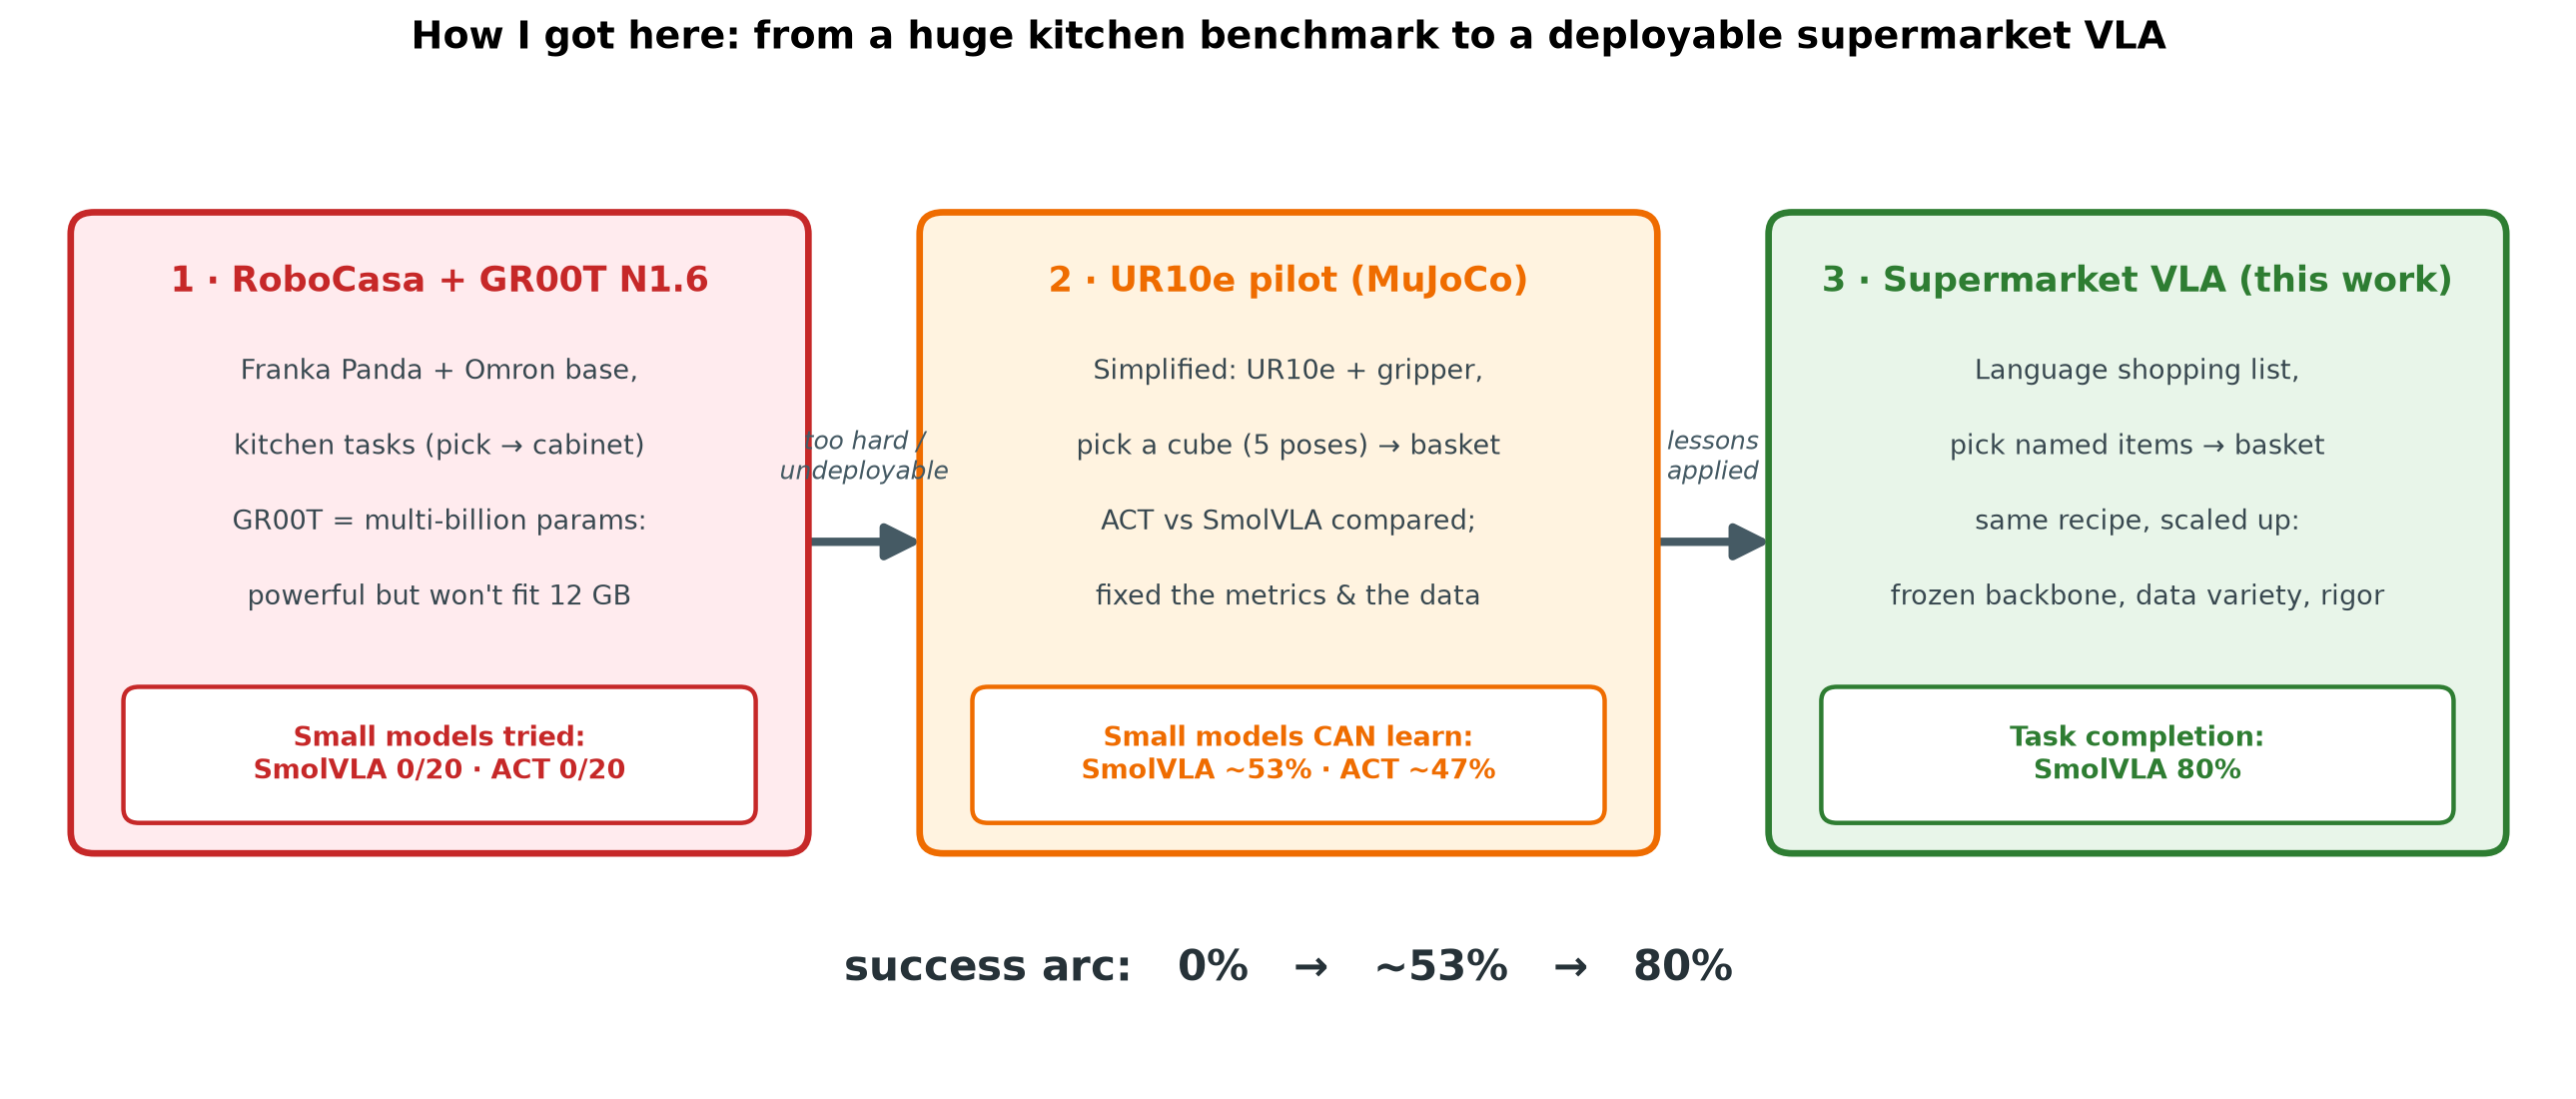
\includegraphics[width=\textwidth,
    alt={A three-stage progression diagram: RoboCasa with GR00T (small models 0 percent), the UR10e pilot (about 53 percent), and the supermarket VLA (80 percent), linked by arrows.}]{figures/journey_prior_work}
\end{center}
\caption{The progression of the project: a large model works on RoboCasa but is
undeployable; small models fail the benchmark; a controlled UR10e pilot succeeds;
the lessons scale to the supermarket task. Success rate rises 0\% $\rightarrow$
$\sim$53\% $\rightarrow$ 80\%.}
\label{fig:journey}
\end{figure}

\begin{figure}[ht]
\begin{center}
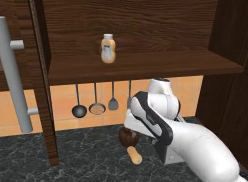
\includegraphics[width=0.32\textwidth,
    alt={The RoboCasa Franka robot doing a kitchen task.}]{figures/prog_robocasa}\hfill
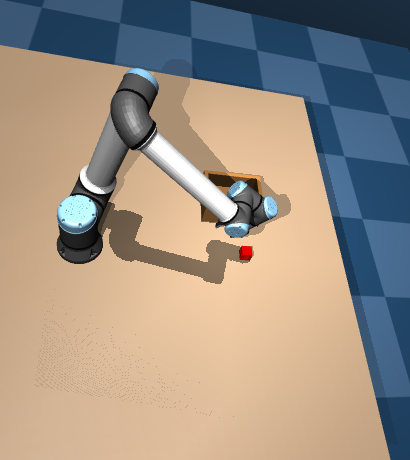
\includegraphics[width=0.32\textwidth,
    alt={The UR10e arm picking a cube on a table in the pilot study.}]{figures/prog_ur10e}\hfill
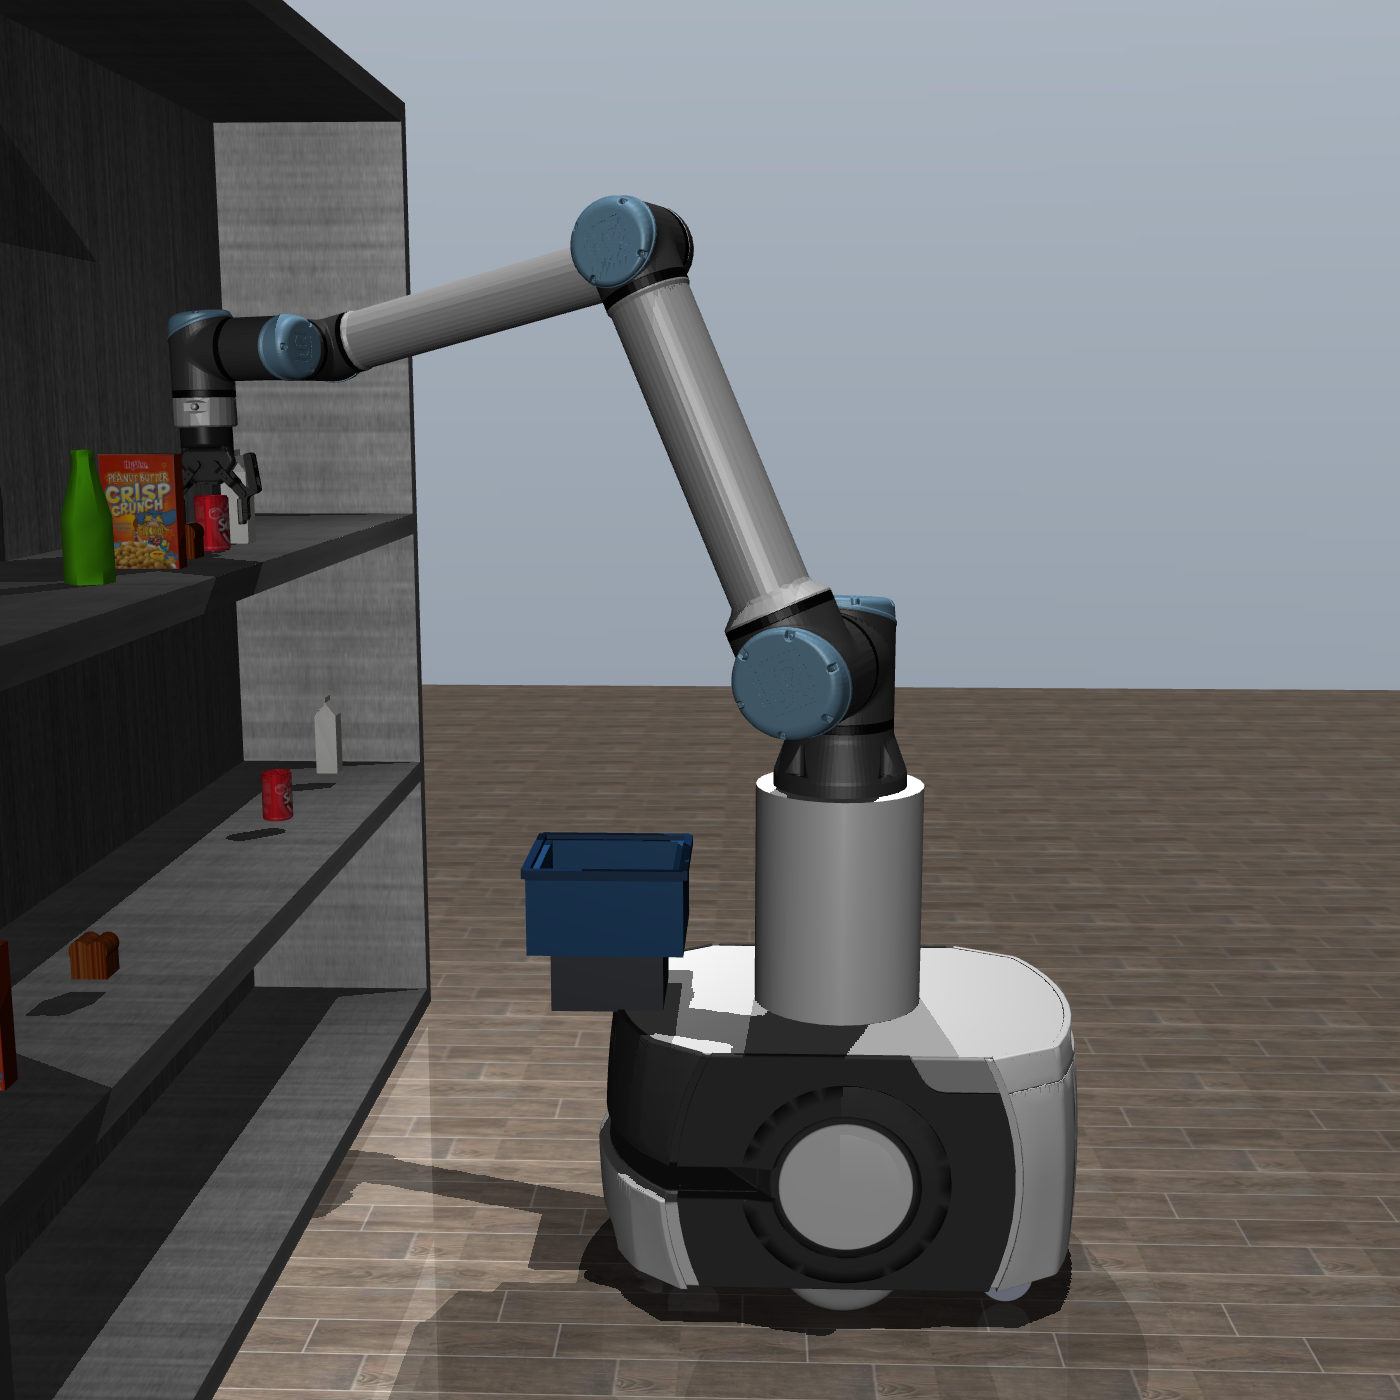
\includegraphics[width=0.32\textwidth,
    alt={The supermarket mobile manipulator at the shelf.}]{figures/prog_supermarket}
\end{center}
\caption{The three robots, left to right: RoboCasa (Franka on a mobile base,
GR00T~N1.6); the fixed-base UR10e pilot; and the supermarket mobile manipulator
studied in this thesis.}
\label{fig:robots}
\end{figure}

\section{Headline result}
\label{sec:results-headline}
On the supermarket task, the fine-tuned SmolVLA policy (best checkpoint; see
\refsec{sec:results-checkpoint}) achieves an \textbf{80\% task-completion rate}
(95\% Wilson CI 70--87) and a \textbf{92.5\% grasp success rate}, measured over
\textbf{320 closed-loop trials} (four items, 20 trials each, across four
checkpoints; the best-checkpoint headline aggregates its 80 item-trials with the
per-item detail below). The result is not a single fortunate demonstration but an
aggregate over many trials with confidence intervals throughout.

This figure should be read against two reference points. Kiviranta reports an 80\%
single-task success rate fine-tuning the same SmolVLA checkpoint on real SO-101
hardware from around 100 demonstrations \cite{kiviranta2025smolvla}, so the result
here is in the same regime as an independent study on real hardware, obtained under a
strict 12~GB budget and with a language-conditioned choice among four items rather
than a single fixed task. The second reference point is internal: the same family of
small models scored 0/20 on the RoboCasa benchmark (\refsec{sec:results-journey}), so
the 80\% here reflects not a change of model but the controlled task and the
disciplined methodology built around it. Together these answer RQ1 affirmatively --- a
compact VLA is deployable on a single consumer GPU at a useful success rate --- while
the remainder of the chapter examines \emph{why} it works and where it does not.

\section{Per-item results}
\label{sec:results-peritem}
\reftab{tab:peritem} and \reffig{fig:peritem} give the per-item breakdown for the
selected checkpoint. Three of the four items complete at or above 75\%, and two at
or above 90\%; grasping is essentially solved for three items at 100\%. The milk
carton is the weakest item, which is analysed in \refsec{sec:disc-limits}.

\begin{table}[ht]
\caption{Per-item grasp and task-completion (placement) rates for the selected
checkpoint, with $n=20$ trials per item and Wilson 95\% confidence intervals on the
placement rate.}
\begin{center}
\tagpdfsetup{table/header-rows={1}}
\begin{tabular}{lccc}
\toprule
Item & Grasp & Placed (task complete) & 95\% CI \\
\midrule
Cola can      & 100\% & 95\% & 76--99 \\
Water bottle  & 100\% & 90\% & 70--97 \\
Bread loaf    & 100\% & 75\% & 53--89 \\
Milk carton   & 70\%  & 60\% & 39--78 \\
\midrule
Overall       & 92.5\% & 80\% & 70--87 \\
\bottomrule
\end{tabular}
\end{center}
\label{tab:peritem}
\end{table}

\begin{figure}[ht]
\begin{center}
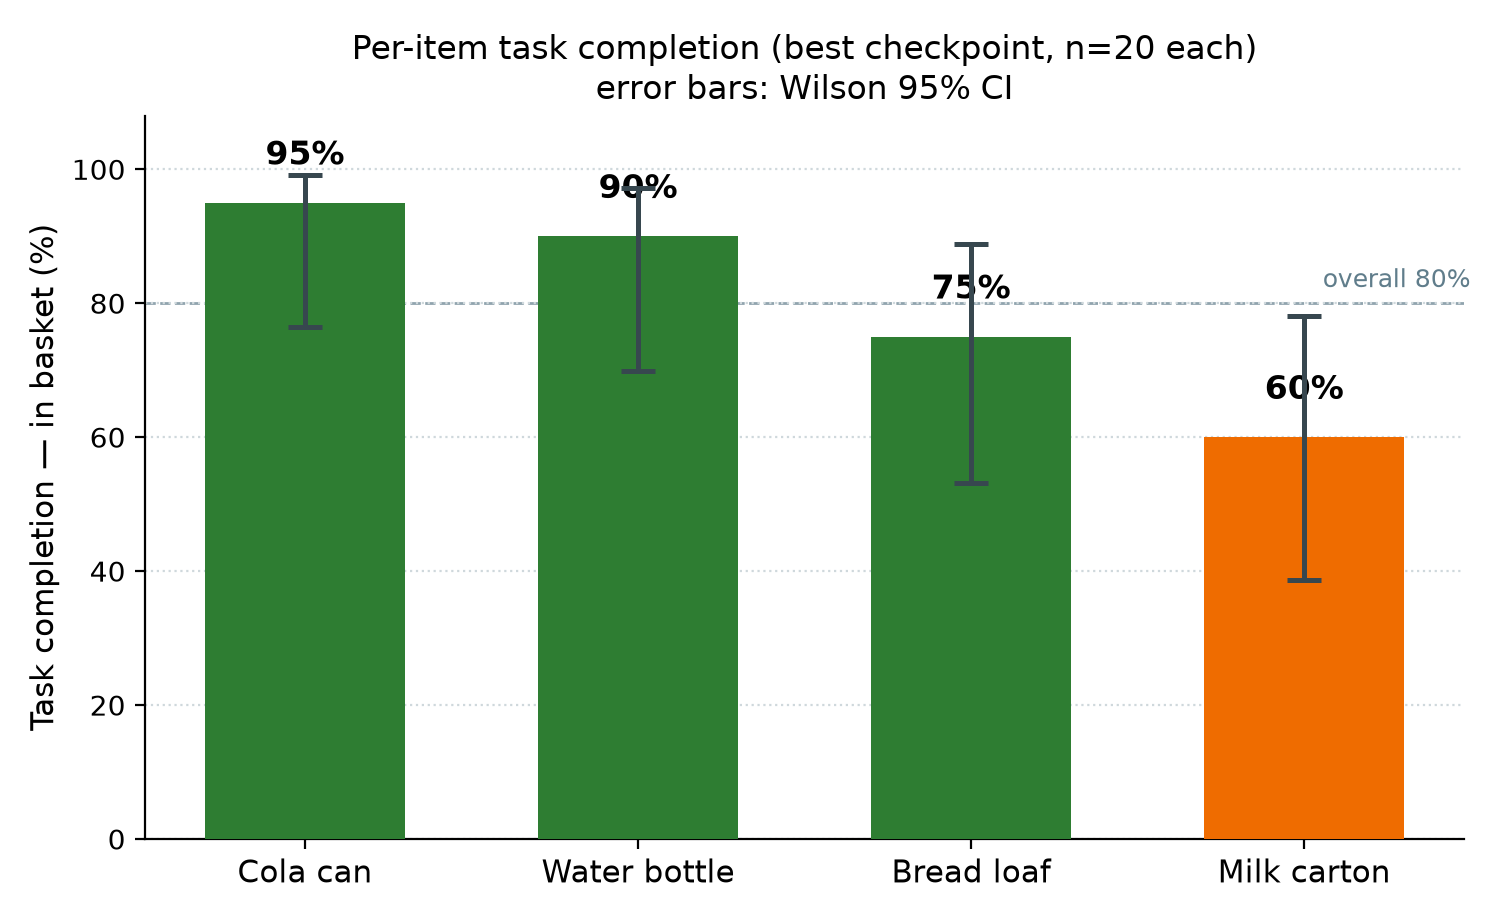
\includegraphics[width=0.8\textwidth,
    alt={A bar chart of per-item task-completion rates with Wilson confidence-interval error bars: cola 95 percent, water bottle 90 percent, bread 75 percent, milk 60 percent.}]{figures/per_item_success}
\end{center}
\caption{Per-item task-completion rate for the selected checkpoint, with Wilson
95\% confidence-interval error bars ($n=20$ each). The dashed line marks the 80\%
overall rate.}
\label{fig:peritem}
\end{figure}

The per-item pattern is informative. The \textbf{cola can} and \textbf{water
bottle} are the strongest items (95\% and 90\% placement, both 100\% grasp): the can
is compact and easy to grip, and the bottle, although tall, sits at the near-side
reach where the wrist camera has a clean view during the descent, and its higher grip
point (\refsec{sec:m-grasp}) gives a stable hold. The \textbf{bread loaf} grasps
perfectly (100\%) but places slightly less reliably (75\%), consistent with its
larger footprint making the final drop into the tote more sensitive to lateral
error. The \textbf{milk carton} is the clear outlier (70\% grasp, 60\% placement).
Its weakness has two causes, neither of them kinematic reach. First, it is the tallest
item on the shelf, so its peak lift clears the \SI{0.05}{m} grasp threshold by the
smallest margin of any item (median \SI{0.054}{m}); the grasp metric is therefore
least reliable precisely for this item, and its 70\% figure is better read as a lower
bound than as a measurement. Second, the learned reach exhibits a consistent inward
bias: all four items are approached slightly short of their true lateral position,
toward the shelf centre, so the items furthest from the centre are approached least
accurately. Note that the milk carton is \emph{not} the most extended target --- the
water bottle sits \SI{8}{cm} further from the centreline (\refsec{sec:m-env}) and
achieves 100\% grasp --- and the scripted expert reaches 98\% on the carton with no
item-specific tuning, so the difficulty lies in the learned policy rather than in the
robot's kinematics. That the
milk carton placed more reliably at earlier checkpoints (\refsec{sec:results-checkpoint})
indicates the weakness is not intrinsic to the item but an artefact of where in
training the deployed checkpoint was taken, and is therefore recoverable
(\refsec{sec:disc-limits}). The overall separation between a near-solved grasp phase
and a more variable placement phase --- 92.5\% versus 80\% --- localises the residual
difficulty to the final drop rather than to perception or reaching, a theme returned
to in the failure analysis below.

\section{Failure analysis: from 0\% to 80\%}
\label{sec:results-diagnosis}
The first policy trained on the supermarket task placed items \emph{0\%} of the
time (0 of 12 trials; grasp 9 of 12). That baseline rests on a much smaller sample
than the 80 trials per checkpoint reported above --- a 0/12 result carries a Wilson
95\% confidence interval of roughly 0--24\% --- so the comparison with the final
figure should be read as an order-of-magnitude improvement rather than an exact
80-point gain. Rather than assume a broken policy, a single episode was traced in
detail.
The policy in fact performed the whole task --- grasping the item, carrying it, and
lowering it to within about two centimetres of the basket --- before (a) releasing
about ten centimetres short, so the item rolled out of the small basket, and
(b) failing to stop cleanly, swinging back toward the shelf and occasionally
knocking the item out. The failure was therefore one of \emph{final-drop precision
and observability}, not of task understanding: perception, language, grasping and
transport all worked. \reffig{fig:nearmiss} depicts this failure mode
schematically.

\begin{figure}[ht]
\begin{center}
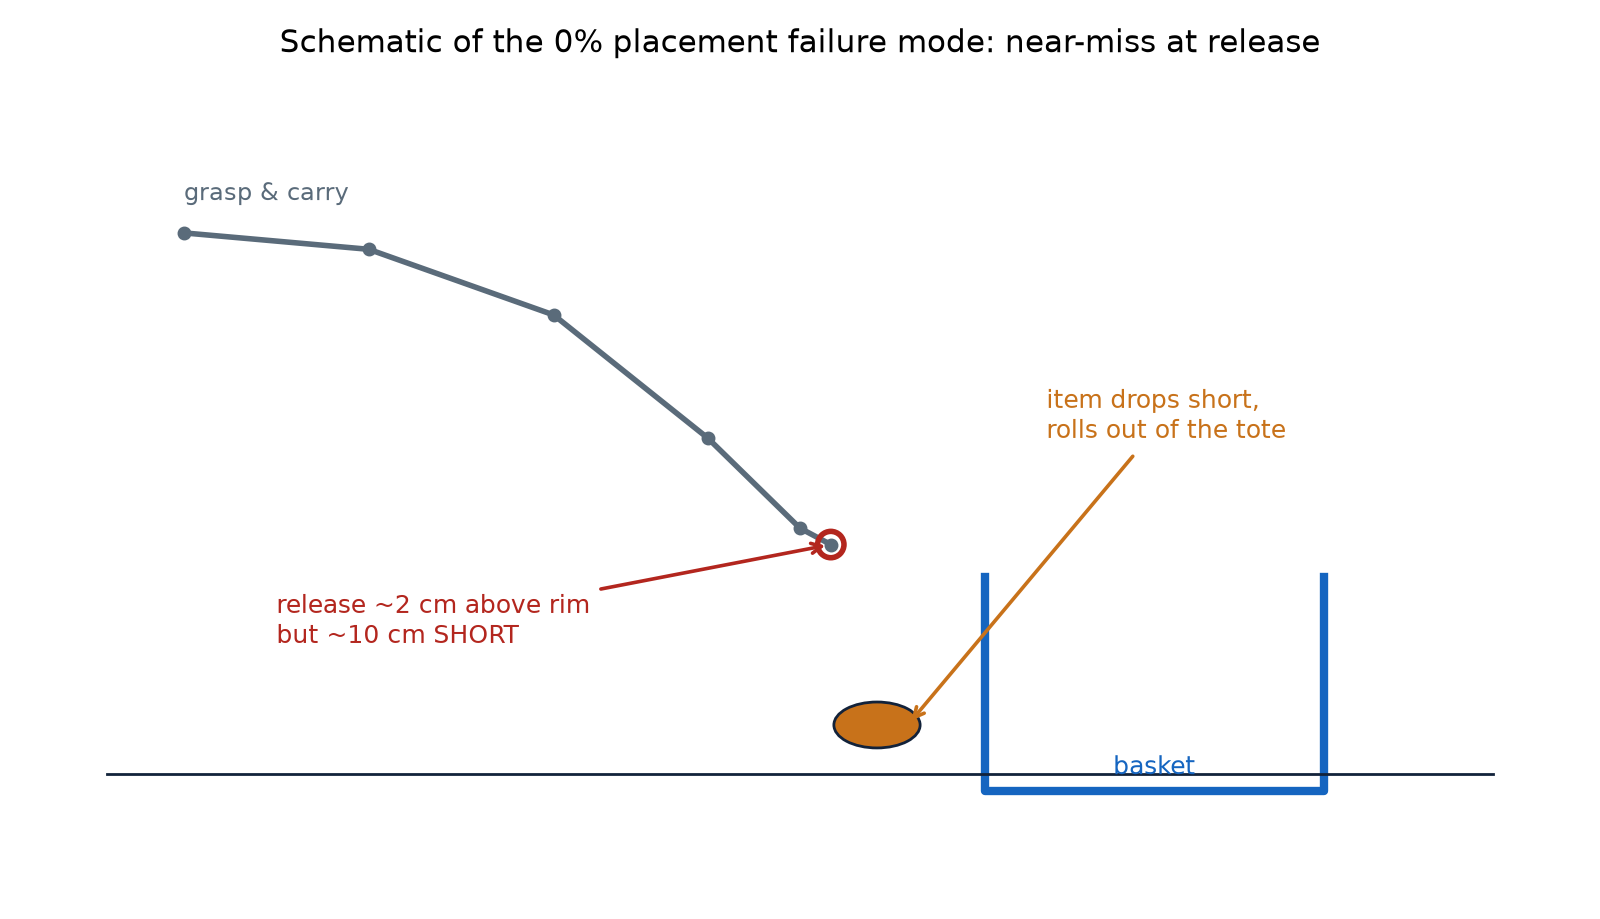
\includegraphics[width=0.8\textwidth,
    alt={A side-view schematic of the near-miss failure: the gripper carries and lowers the item but releases about ten centimetres short of the basket, so the item drops short and rolls out.}]{figures/fig_nearmiss}
\end{center}
\caption{Schematic of the initial 0\% placement failure. The policy grasps,
carries and lowers the item to just above the rim height, but releases
approximately ten centimetres short of the basket, so the item drops outside the
tote and rolls away --- a near-miss, not a failure of task understanding.}
\label{fig:nearmiss}
\end{figure}

This diagnosis pointed to three targeted changes, none of which involved scaling
the model: (i) \emph{clean episode boundaries} in the demonstrations, ending each
demo at placement so the policy is not taught to move away after releasing;
(ii) a \emph{dedicated basket camera} (\reffig{fig:basketcam}), because the policy
could previously barely see the drop target; and (iii) a \emph{wider basket} that
tolerates the residual near-miss. Together these raised placement from 0\% to 80\%.

Each fix targets a distinct facet of the diagnosis. The \emph{clean episode
boundary} is a data correction: by ending every demonstration at the moment of
placement, the policy is no longer shown the return-to-home motion and therefore does
not learn to move away immediately after releasing, which had been re-opening the
grip near the shelf and dislodging the item. The \emph{basket camera} is an
observability correction: previously the tote was visible only obliquely and late,
through the wrist and scene views, so the policy had little signal with which to
judge the final centimetres of the descent; a dedicated view of the drop target
supplies exactly that signal throughout the carry and release. The \emph{wider tote}
is a tolerance correction: it enlarges the target footprint so that the residual
lateral error at release --- which the other two fixes reduce but do not eliminate ---
still lands the item inside. It is worth emphasising that none of these changes
increases the model's capacity; the gain comes entirely from what the policy is
taught, what it can see, and how forgiving the target is. This is the central answer
to RQ4: the initial failure was a specific, localisable defect at the end of the
motion, and it was corrected by diagnosis rather than by scale.

\begin{figure}[ht]
\begin{center}
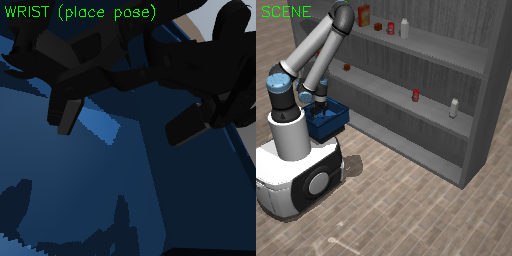
\includegraphics[width=0.49\textwidth,
    alt={The basket seen poorly from the wrist camera before the fix.}]{figures/basket_visibility}\hfill
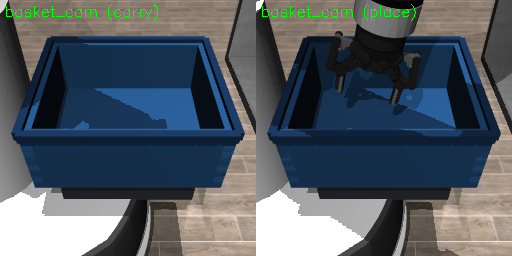
\includegraphics[width=0.49\textwidth,
    alt={The dedicated basket camera providing a clear view of the tote and the gripper descending into it.}]{figures/basket_cam}
\end{center}
\caption{Motivation and fix for the placement failure. Left: the basket is poorly
visible from the existing views. Right: the added basket camera gives a clear view
of the drop target throughout the carry and release.}
\label{fig:basketcam}
\end{figure}

\section{Language grounding}
\label{sec:results-language}
To test whether the policy genuinely uses the instruction rather than executing a
fixed motion, the scene was held constant and only the instruction word was
changed. \reftab{tab:grounding} reports the gripper's lateral ($y$) position at
the reach, against the target item's true position. The arm reaches the
\emph{named} item --- left for milk, centre for bread, right for the water bottle
--- so the target moves with the word. This is genuine language grounding, not a
memorised trajectory; the graded per-item success rates in
\reftab{tab:peritem} are likewise the signature of a learned controller rather than
a lookup.

The design of this test is deliberately adversarial to the null hypothesis. If the
policy had learned a single fixed reaching motion --- ignoring the instruction and
exploiting, say, the most salient object --- then changing only the words would leave
the reach unchanged, and the reached position would be constant across the three
instructions. Instead the reached lateral position tracks the named item across the
full width of the shelf, from $-0.24$ to $+0.29$\,\si{m}, a span far larger than the
few-centimetre residual error, so the instruction is demonstrably the causal variable.
This matters because language conditioning is the property that distinguishes a VLA
from the non-VLA ACT baseline (\refsec{sec:bg-act}) and is, per
\textcite{kiviranta2025smolvla}, easy to claim but fragile in practice; verifying it
with a controlled intervention rather than assuming it is therefore central to
answering RQ3. The small systematic undershoot on the far item (reaching $+0.29$ for a
target at $+0.34$) belongs to the \emph{water bottle}, not the milk carton, which sits
at $-0.26$. It is not specific to that item: all four items are reached slightly short
of their true lateral position, a consistent inward bias toward the shelf centre. Such
a bias is characteristic of a policy interpolating between demonstrated trajectories
rather than localising each item independently, and reflects reduced precision at the
extremes of the demonstrated range rather than a failure of grounding.

\begin{table}[ht]
\caption{Language-grounding test. With the scene fixed and only the instruction
changed, the gripper reaches the named item's lateral position.}
\begin{center}
\tagpdfsetup{table/header-rows={1}}
\begin{tabular}{lcc}
\toprule
Instruction & Item's $y$ (m) & Gripper reached $y$ (m) \\
\midrule
``milk carton''  & $-0.26$ & $-0.24$ \\
``loaf of bread'' & $\phantom{-}0.00$ & $-0.01$ \\
``water bottle'' & $\phantom{-}0.34$ & $\phantom{-}0.29$ \\
\bottomrule
\end{tabular}
\end{center}
\label{tab:grounding}
\end{table}

\section{Checkpoint selection}
\label{sec:results-checkpoint}
\reftab{tab:checkpoints} and \reffig{fig:checkpoints} report the closed-loop
performance of all four saved snapshots, evaluated over 80 trials each. The
15{,}000-step checkpoint attains the highest task-completion rate at 80\%, and was
the one deployed.

The differences between checkpoints must, however, be interpreted with care. Because
every checkpoint was evaluated on the same trial seeds, the trials are paired and
McNemar's exact test applies. Applied to task completion, \emph{no} pair of
checkpoints differs significantly (all $p \ge 0.19$ uncorrected, and all $p = 1.00$
after Holm correction for the six pairwise comparisons). On the grasp sub-task the
picture is different: grasp success at 15k is significantly better than at 5k
($p = 0.008$; Holm-corrected $p = 0.048$), while the remaining comparisons do not
survive correction. The defensible conclusion is therefore narrow: training beyond
5{,}000 steps measurably improves \emph{grasping}, but the four checkpoints are
statistically indistinguishable on end-to-end task completion at $n=80$. The apparent
\SI{5}{\percent} dip from 15k to 20k is within sampling noise and should not be read
as over-training; a per-item breakdown (\reftab{tab:peritemckpt}) shows it is driven
almost entirely by a single item, the water bottle, rather than being a consistent
regression.

A further consideration is that the learning-rate schedule was configured for
30{,}000 decay steps but training was stopped at 20{,}000
(Appendix~\ref{app:Implementation}), so the cosine decay was truncated at roughly two-thirds
of its intended course and the learning rate at 15k was still $1.68\times10^{-5}$,
about 17\% of peak. None of the checkpoints represents a converged endpoint.

The methodological point stands independently of the ranking, and is what matters for
RQ2: closed-loop task success and the training objective are not monotonically
related, so the decision of which snapshot to deploy must be made on measured
behaviour rather than on the training signal. Here that choice was consequential only
in the weak sense that the final checkpoint was not the empirical best.

\begin{table}[ht]
\caption{Overall task-completion rate by training checkpoint ($n=80$ each), with
Wilson 95\% confidence intervals. The 15k checkpoint is selected.}
\begin{center}
\tagpdfsetup{table/header-rows={1}}
\begin{tabular}{lcc}
\toprule
Checkpoint (steps) & Task completion & 95\% CI \\
\midrule
5{,}000  & 68.8\% & 58--78 \\
10{,}000 & 68.8\% & 58--78 \\
\textbf{15{,}000} & \textbf{80.0\%} & \textbf{70--87} \\
20{,}000 & 75.0\% & 65--83 \\
\bottomrule
\end{tabular}
\end{center}
\label{tab:checkpoints}
\end{table}

\begin{table}[ht]
\caption{Placement success per item and per checkpoint ($n=20$ per cell). The
\SI{5}{\percent} aggregate drop from 15k to 20k is not consistent across items: the
milk carton improves by four trials and the bread loaf is unchanged, while the water
bottle accounts for the entire decline.}
\begin{center}
\tagpdfsetup{table/header-rows={1}}
\begin{tabular}{lccccc}
\toprule
Checkpoint & Cola can & Water bottle & Milk carton & Bread loaf & Overall \\
\midrule
5{,}000  & 90\% & 50\% & 85\%  & 50\% & 68.8\% \\
10{,}000 & 95\% & 30\% & 100\% & 50\% & 68.8\% \\
\textbf{15{,}000} & 95\% & 90\% & 60\% & 75\% & \textbf{80.0\%} \\
20{,}000 & 90\% & 55\% & 80\%  & 75\% & 75.0\% \\
\midrule
Change 15k$\rightarrow$20k & $-1$ & $\mathbf{-7}$ & $+4$ & $0$ & $-4$ \\
\bottomrule
\end{tabular}
\end{center}
\label{tab:peritemckpt}
\end{table}

\begin{figure}[ht]
\begin{center}
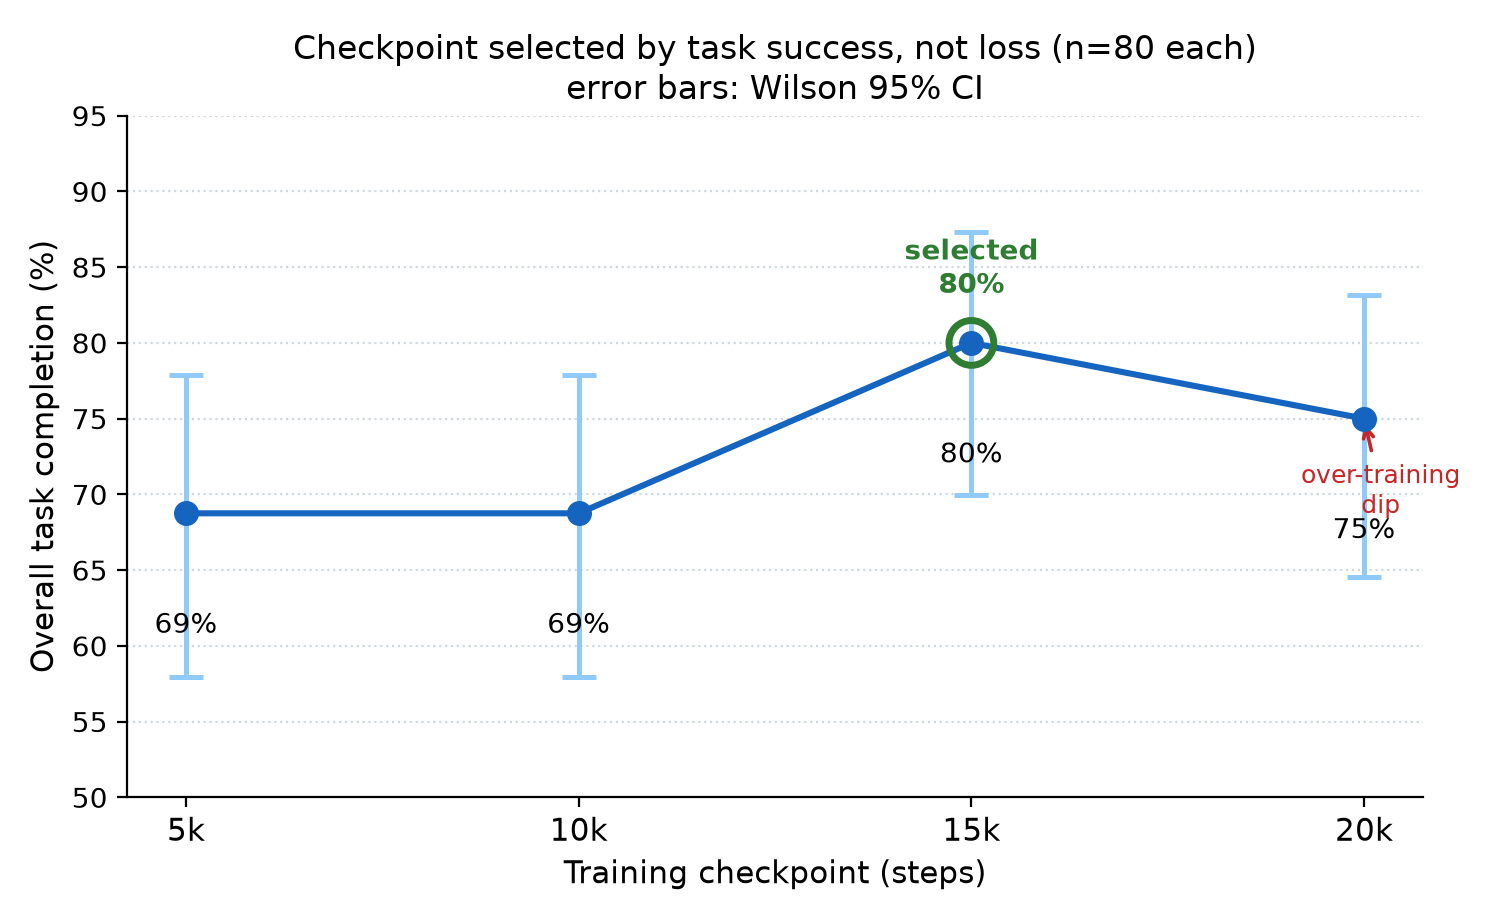
\includegraphics[width=0.8\textwidth,
    alt={A line chart of task-completion rate versus training step, peaking at the 15k checkpoint (80 percent) and dipping at 20k (75 percent), with confidence-interval error bars.}]{figures/checkpoint_selection}
\end{center}
\caption{Task-completion rate versus training checkpoint, selected by closed-loop
success rather than loss. The 15k checkpoint attains the highest rate; the
differences between checkpoints are not statistically significant at $n=80$
(McNemar, all $p \ge 0.19$), so the error bars should be read as overlapping.}
\label{fig:checkpoints}
\end{figure}

\section{Interpretability: the model's predicted plan}
\label{sec:results-interpret}
Because SmolVLA predicts a chunk of 50 future actions, the model's own plan can be
surfaced at each re-planning step. At the very first frame of an episode --- with
the arm still at its home pose, far from the item --- the predicted gripper channel
already transitions to ``closed'' at approximately step~16. In other words, the
policy has decided \emph{to grasp} before it has reached the object. This readout
is decoded directly from the network's output rather than from any hand-written
heuristic, and provides a small but genuine window into the policy's intention.

This behaviour is consistent with the role of action chunking discussed in
\refsec{sec:bg-vla}: by committing to a temporally extended plan rather than a single
next action, the policy encodes an anticipatory intention --- to grasp --- before the
sensory evidence that the item is within reach. It also makes the placement phase
interpretable: as the gripper approaches the basket, the planned gripper channel
transitions back to ``open'' a fixed number of steps ahead of the physical release,
so the moment of intended release can be read from the plan before it occurs. Beyond
its explanatory value, such a readout is practically useful as a lightweight monitor:
a plan that never intends to close, or intends to release while far from the basket,
flags a likely failure before it happens, without any additional model or label.

This form of interpretability is worth distinguishing from post-hoc explanation
methods that attribute a decision to input features after the fact. Here the ``plan''
is not an approximation or a saliency map but the model's literal output --- the
sequence of actions it will execute unless it re-plans --- so reading it involves no
additional assumptions and no auxiliary model. It is admittedly a narrow window: it
reveals what the policy intends to do, not why it intends to do it, and it does not
expose the visual features driving the decision. Nonetheless, for a safety-relevant
system the ability to read a short-horizon intention directly from the controller is
valuable, and it comes for free from the action-chunking design. In the two-VLA vision
of \refsec{sec:future}, an analogous readout of the navigation policy's planned path
would be a natural and cheap safety monitor around moving people.

\section{End-to-end shopping list}
\label{sec:results-orchestrator}
Finally, an orchestrator sequences single-item picks into a shopping list. The user
selects items from a menu of the available products; the robot collects them in
order, with the basket accumulating items across picks (the scene is reset once at
the start, not between items), and re-attempts an item if it misses. This
demonstrates the intended end-to-end behaviour: a language/menu request in,
collected items out.

A caveat observed empirically is that multi-item completion is lower than the
product of the single-item rates would predict. When the first item is already in
the basket, the scene and basket cameras show a configuration the policy never saw
during training (which always began with an empty basket), and this
out-of-distribution view degrades the subsequent pick --- the far-edge water bottle
being the most sensitive. The first item of a list is therefore always as reliable
as the single-item rates in \reftab{tab:peritem}; later items are somewhat less so.
The menu interface (which constrains the request to the known catalogue) and the
retry-on-miss behaviour mitigate this, but the underlying distribution shift is a
data problem, analysed with its remedy in \refsec{sec:disc-limits}.

Two design choices in the orchestrator are worth noting. First, item selection is
made through a fixed menu of the known products rather than by parsing arbitrary free
text; this is a deliberate reliability decision, since the language competence that
matters for the task is grounding a named item in the scene (which the policy does),
not open-vocabulary parsing (which it was not trained for and which a small brittle
parser would get wrong). Second, between items the arm is returned to its home
configuration --- the same start state used during data collection --- so that each
pick begins in-distribution; the scene, however, is not reset, so previously collected
items genuinely accumulate in the basket. The retry-on-miss policy re-attempts a
dropped item a bounded number of times, which recovers many of the stochastic
single-attempt failures at the cost of additional time. Together these make the
orchestrator a faithful end-to-end demonstration of the intended behaviour while
keeping its failure modes attributable to the underlying policy rather than to the
sequencing layer.

\section{Synthesis}
\label{sec:results-synthesis}
Taken together, the results support three claims. First, a compact VLA is
\emph{deployable} under a hard 12~GB budget and reaches a useful 80\% task-completion
rate on this task (\refsec{sec:results-headline}). Second, the largest gains came
from \emph{methodology rather than scale}: the 0\%-to-80\% improvement
(\refsec{sec:results-diagnosis}) followed from diagnosis and from correcting
observability, data boundaries and the target, not from a larger model; and the
prior pilot showed metric and data fixes dominating model choice
(\refsec{sec:results-journey}). Third, the policy is genuinely
\emph{instruction-following} rather than executing a fixed motion
(\refsec{sec:results-language}), and its behaviour is partly \emph{legible} through
its own predicted plan (\refsec{sec:results-interpret}). The clear separation
between a near-solved grasp phase (92.5\%) and a more variable placement phase
(80\%) localises the remaining difficulty to final-drop precision under a stochastic
policy --- precisely the regime the evaluation protocol was designed to measure
honestly.

Read against the research questions of \refsec{sec:rqs}, the chapter answers each in
turn. RQ1 (feasibility) is answered affirmatively by the 80\% headline under a strict
12~GB budget. RQ2 (model versus methodology) is answered by two independent pieces of
evidence: the pilot, where fixing the metric and the data --- not the model --- moved
real performance from an apparent 80\% to a real 40\% and then upward; and the
supermarket task, where the decisive 0\%-to-80\% gain came from observability and data
fixes rather than scale, and where even checkpoint selection had to be made by task
success rather than loss. RQ3 (grounding) is answered by the controlled
instruction-swap test, in which the reach follows the named item across the shelf. RQ4
(failure structure) is answered by the traced diagnosis, which localised the initial
failure to the terminal placement and corrected it by targeted changes. That all four
questions admit clear, evidence-based answers is itself a result: it is a consequence
of designing the evaluation, from the outset, to make such answers possible rather than
to maximise a single headline number.

\chapter{Discussion}
\label{chap:discussion}

\section{Interpretation}
\label{sec:disc-interp}
The central finding of this thesis is that a compact VLA can be fine-tuned and
deployed within a 12~GB GPU budget to perform a language-conditioned manipulation
task with an 80\% task-completion rate. Two aspects of \emph{how} that result was
obtained are as important as the number itself.

First, the largest improvements came from \emph{methodology, not model scale}. The
preliminary study (\refsec{sec:results-journey}) showed that fixing a success-metric
bug and removing duplicated demonstrations moved real performance far more than any
architectural change, and the supermarket result was reached with a
\emph{frozen} backbone and only 208 training demonstrations. This is consistent with the
literature: $\pi_{0.5}$ and RoboAgent both attribute performance to data diversity
and composition rather than to scaling the action model alone
\parencite{black2025pi05, bharadhwaj2024roboagent}. The frozen-backbone strategy
also validates the pretrain-then-post-train view \parencite{xiang2026posttraining}:
the model arrives already knowing what the objects are and what the words mean, and
fine-tuning need only supply the motor mapping --- which is why so few
demonstrations sufficed.

Second, the 0\%-to-80\% improvement (\refsec{sec:results-diagnosis}) came from
\emph{diagnosis rather than brute force}. Tracing a single failure revealed that
the policy already understood the task and was near-missing at the final drop; the
fixes targeted observability and episode boundaries specifically. This is a more
transferable outcome than a number obtained by simply retraining a larger model.

The language-grounding test (\refsec{sec:results-language}) confirms that the
policy is genuinely instruction-following: with the scene fixed, changing only the
instruction word moves the reach to the named item. Together with the graded
per-item success rates, this rules out the hypothesis that the policy executes a
\emph{single} memorised trajectory irrespective of the instruction.

It does not, however, rule out the hypothesis that the policy executes \emph{one
memorised trajectory per item word}, and \refsec{sec:results-lookup} shows that this
is what it does. The distinction is the most consequential finding of this thesis, and
it is worth being precise about why the weaker test was insufficient. Every item
occupied a fixed position in all 208 training episodes and in the grounding test
itself; under those conditions ``localise the named object and reach to it'' and
``recall where that word's object sits and reach there'' are behaviourally identical.
Only moving the objects separates them, and when they are moved the policy follows the
recalled position without exception. The lesson generalises beyond this thesis: a
grounding test conducted on a positionally static scene cannot establish grounding, no
matter how cleanly the reach tracks the instruction, and results of that form in the
wider literature should be read with the same reservation. That this thesis's own
earlier claim did not survive the stronger test is an argument for running it.

The success of the frozen-backbone strategy deserves emphasis, because it reframes
what fine-tuning a VLA on a small dataset actually involves. The intuition that a
policy must ``learn to see'' the objects is misleading in this setting: the backbone
already sees and reads competently from its pretraining, and the 208 training demonstrations
supply only the missing ingredient --- how this particular embodiment should move to
act on what is already perceived. This division of labour is what makes the data
requirement so modest, and it explains why an attempt to retrain the perception on so
few examples was not merely unnecessary but actively harmful in the pilot, where it
either exhausted memory or destabilised training. The broader lesson is that, under
constraint, the right question is not ``how much of the model can I train?'' but ``how
little of it \emph{must} I train?''. Identifying the smallest sufficient set of
parameters to adapt --- here, the action expert alone --- is both a memory strategy and a
regularisation strategy, and it is a transferable principle for fine-tuning large
pretrained models on limited data in general, not only for this task.

A final interpretive point concerns the decomposition of the task into grasping and
placing. The results consistently show grasping to be the more nearly solved
sub-problem (92.5\% overall, 100\% on three of four items) and placing to be the more
variable one (80\% overall). This is initially counter-intuitive, since grasping ---
aligning a gripper with an object and securing it --- is usually considered the harder
manipulation primitive. The explanation is specific to this task: the grasp is
executed close to the item with a clear eye-in-hand view and benefits directly from
the scripted expert's carefully tuned per-item poses, whereas the placement is a
release into a small target at the end of a longer, stochastic motion, where residual
error has accumulated and (before the basket camera) observability was poorest. The
implication is that, for this class of task, the marginal engineering effort is better
spent on the terminal placement --- its observability, its target tolerance, and the
data around it --- than on the grasp, and this is precisely where the 0\%-to-80\% fixes
were directed. It is a small but useful design heuristic that generalises beyond the
present system: instrument and ease the least-observed, highest-variance phase of the
motion first.

\section{Limitations}
\label{sec:disc-limits}
This work has clear and honestly stated limitations.

\subsection{Weak item.} The milk carton is the weakest item (70\% grasp, 60\%
placement). It is the tallest item, so its peak lift clears the grasp threshold by the smallest margin of any item, and the learned reach exhibits a consistent inward bias (Sec. 4.3). It is not the most laterally extended target — the water bottle sits 8 cm further out and grasps at 100 \%. It placed more reliably at earlier checkpoints, so the weakness is recoverable with milk-specific grasp tuning or additional milk demonstrations rather than being fundamental.

\subsection{Multi-item lists.} Single-item picks are reliable, but whole-list
completion is not: 45\% for two items and 30\% for three
(\refsec{sec:results-orchestrator}). An accumulating basket was previously assumed to
be the cause, on the reasoning that the policy never saw a non-empty basket in
training. Measurement does not support this: success does not decline as the basket
fills. The mechanism remains open, and the most plausible candidate is the one
identified in \refsec{sec:results-lookup} --- earlier picks nudge the remaining items,
and a policy that reaches a recalled position rather than a perceived one fails once
its target has moved.

\subsection{Reliance on fixed object positions.} The policy does not localise the named
item; it recalls where that item was demonstrated (\refsec{sec:results-lookup}). This
is the root cause behind several entries in this list, including the \SI{2.5}{cm}
robustness result and, most likely, the multi-item degradation above. It is a data
limitation rather than a model limitation: with every item at a fixed position in all
208 episodes, a word-to-trajectory association fits the demonstrations exactly and is
far simpler to learn than visual search, so the training set never gave the policy a
reason to look. The direct remedy --- re-collecting demonstrations with item positions
randomised over a substantial range, so that the recalled-position strategy no longer
fits the data --- is the single highest-value next experiment this work suggests, and is
developed in \refsec{sec:disc-ideal}.

\subsection{Excluded item.} The cereal box is excluded from training because its
wide face slips in the two-finger gripper during transport; a wider grasp or a
different grip strategy would be required.

\subsection{Simulation only.} All results are in simulation; no sim-to-real transfer
is claimed. The pipeline is deliberately real-robot-shaped, however --- it uses the
LeRobot framework and accurate hardware models (UR10e, Robotiq) --- so the same
code path could fine-tune on real demonstrations.

\subsection{Stochastic policy.} The flow-matching action expert samples actions
stochastically, so there is run-to-run variance, especially on the weak items. This
is exactly why success is reported over 320 trials with confidence intervals rather
than from single runs.

\subsection{Checkpoint selection.} Checkpoints are selected by closed-loop success on
evaluation episodes that use fresh seeds and paraphrases but the same item set; a
fully locked, never-used-for-selection test set would be a cleaner final estimate.

\subsection{Inference cost and control rate.} Although the frozen-backbone strategy
makes \emph{training} inexpensive, \emph{inference} still runs the full
vision--language backbone every re-planning step, which bounds the achievable control
rate on modest hardware. This is acceptable for the quasi-static manipulation task
studied here, where the environment does not change during a pick, but it would be a
first-order concern for the dynamic navigation stage, where a slow control loop is
unsafe around moving people. This is a further, concrete argument for the dual-system
architecture discussed in \refsec{sec:disc-ideal}, in which only a small reflex policy
need run at high rate. The action-chunk horizon is a further lever: executing more of
each predicted chunk before re-planning amortises the backbone cost but reduces
reactivity, the non-monotonic trade-off noted in \refsec{sec:bg-eval}.

\subsection{Scope of the instruction set.} The language conditioning is exercised over
six paraphrase templates spanning four items --- 24 distinct instructions; it is not
tested on open-vocabulary requests, unseen object names, compositional instructions
(``the small red can''), or referring expressions that require disambiguation. The
grounding result of \refsec{sec:results-language} should therefore be read as evidence
that the policy uses the instruction to select among four known items, and
\refsec{sec:results-lookup} narrows this further: the selection is among four
memorised behaviours, not among four perceived objects. Neither result supports a
claim of open-world language understanding, which would require the far more diverse
data discussed as future work.

\section{On cross-benchmark evaluation and specialisation}
\label{sec:disc-crosseval}
A natural question is whether the supermarket-fine-tuned policy could be evaluated
directly on the RoboCasa kitchen benchmark, to compare it against the reference
foundation model. It could be run, but the result would not be meaningful, because
fine-tuning specialises the policy to a specific \emph{interface} as well as a
specific task. The action expert and its frozen normalisation statistics are tied to
this project's embodiment: a seven-dimensional action of six UR10e joint targets
plus a gripper command, and three cameras (wrist, scene, basket) at a fixed
resolution and placement. RoboCasa uses a different embodiment (a Franka arm on a
mobile base), a different action convention and dimensionality, and different camera
streams and objects. Feeding RoboCasa observations to this policy and applying its
outputs to a Franka would be an interface mismatch, not a capability test; failure
there would say nothing about the policy's competence, only that it was asked to
speak a language it was never trained in. This is why the meaningful RoboCasa
experiment reported in \refsec{sec:results-journey} is the converse one --- fine-tune
the small models \emph{on} RoboCasa demonstrations and evaluate \emph{on} RoboCasa,
which yielded 0/20 --- and why generalisation of the present policy is better assessed
on held-out variations of its own task (unseen positions, novel paraphrases) than on
a foreign benchmark. Cross-embodiment transfer is a distinct research problem,
addressed in the literature by co-training across embodiments
\parencite{black2025pi05}, and is out of scope here.

\section{Toward a real-world system without constraints}
\label{sec:disc-ideal}
It is worth asking what an ideal system would look like if compute were not a
constraint. Notably, the answer is not simply ``a larger model'': some limits are
physical rather than computational. A very large model cannot run a fast control
loop, which is unsafe around moving people. The field therefore converges on a
\emph{dual-system} design --- a large reasoner (``System~2'') for planning the list
and interpreting a dynamic scene, paired with a small, fast reflex policy
(``System~1'') for real-time control \parencite{nvidia2025gr00t, black2025pi05}.

Beyond the architecture, five changes would most improve a real deployment; each is
motivated directly by a limitation or observation of the present work. The first is
both the cheapest and, on the evidence of \refChap{chap:results}, the most valuable.

\subsection{Positional randomisation in the demonstrations.} The single most
consequential change would require no additional hardware, no larger model and no new
algorithm: re-collect the demonstrations with each item's position randomised over a
substantial range rather than fixed. \refsec{sec:results-lookup} shows that the policy
currently maps each item word to a memorised trajectory, and
\refsec{sec:results-robustness} shows the cost of that --- a \SI{2.5}{cm} displacement
removes more than twenty points of task completion. Neither is a failing of the model:
with every item at a fixed position in all 208 episodes, recall fits the training data
exactly, so the dataset never made visual localisation necessary. Randomising positions
over, say, the full width of the shelf would make the recalled-position strategy
inconsistent with the demonstrations and force the policy to use the visual information
it already receives --- information the scripted expert demonstrably uses, since it
re-solves its grasp inverse kinematics on the settled object position and maintains
96--100\% per-item success under exactly the jitter that defeats the learned policy.
The experiment is inexpensive, since the data-collection pipeline already supports
per-episode jitter and need only have its magnitude increased, and it is the natural
next step for this work. Its outcome would also be informative either way: if
randomisation produces genuine localisation, the limitation is confirmed as one of
data; if it does not, the limitation lies deeper, in the capacity of a frozen backbone
with a small action expert to support visual search.

\subsection{Whole-body control.} Controlling the base and arm as a single system,
rather than parking the base and then moving the arm, would let the robot reach while
repositioning --- extending its effective workspace, reaching around obstacles, and
approaching items from a more favourable base pose. The parked-base assumption made
here simplifies the manipulation problem: every item must be reached from a single
fixed stance, so the policy has one approach geometry per item and no means of
improving it. A whole-body policy would fold base positioning into the same
optimisation as the reach, allowing a poor approach angle to be corrected by moving
rather than by stretching.

\subsection{Tactile and force sensing.} The clearest capability gap in this thesis is
grasping: the milk carton grasps at 70\% and the cereal box is excluded entirely for
slipping. These are difficult to solve from vision alone, because whether the fingers
have secured an object --- and whether it is slipping during transport --- is a contact
property, not a visual one. Tactile or force sensing on the gripper would provide
exactly this signal, enabling closed-loop grip adjustment and slip detection, and is
the most direct route to lifting the weak items and re-admitting cereal.

\subsection{Diverse, co-trained data.} A four-item, single-scene dataset cannot
support the generalisation a service robot requires. The most effective route,
following $\pi_{0.5}$ \parencite{black2025pi05}, is to co-train on a deliberately
heterogeneous mixture --- teleoperation across many stores and items, domain-randomised
simulation, and even human video --- so that the policy learns invariances rather than
memorising a fixed inventory. It would also broaden the scene distribution generally, though note that basket occupancy was measured not to be the cause of the multi-item degradation (Sec. 4.11).

\subsection{Imitation followed by reinforcement.} Behaviour cloning caps a policy at
the quality of its demonstrations; it can, at best, imitate the scripted expert.
Reinforcement-learning fine-tuning on top of the imitation-pretrained policy ---
safely, in simulation --- could discover behaviours the expert never demonstrated, in
particular robust recoveries from the near-misses that dominate the residual failures
here, pushing performance past the demonstration ceiling.

In this framing, the system built in this thesis is the \emph{deployable subset} of
that ideal: the same fundamental recipe --- a pretrained perception prior, a learned
action mapping, and disciplined evaluation --- constrained to what a single GPU and a
modest demonstration budget allow. The value of characterising that subset carefully
is that it establishes what is achievable now, and identifies precisely which
additions --- contact sensing, whole-body control, data diversity, reinforcement ---
would buy the most, and why.

\section{Comparison with related work}
\label{sec:disc-compare}
The 80\% task-completion rate sits in the same regime as Kiviranta's 80\% single-task
success fine-tuning the same SmolVLA checkpoint on real SO-101 hardware from around
100 demonstrations \parencite{kiviranta2025smolvla}. The two figures should not be
equated, however: Kiviranta's is obtained on physical hardware, where object pose,
lighting and contact vary from trial to trial, whereas the figure here is measured in
simulation at a fixed object pose, and falls to 58.8\% once object position is allowed
to vary by \SI{2.5}{cm} (\refsec{sec:results-robustness}). The coincidence of the two
numbers is therefore a coincidence of regime, not of difficulty. The comparison is
nonetheless consistent with that work's caution that SmolVLA's headline numbers are
easy to overstate without careful evaluation --- a caution this thesis addresses
directly through Wilson intervals, adequate sample sizes, success-based checkpoint
selection and, ultimately, by testing and revising its own headline claim. The observation that
data and metrics dominate model choice at this scale aligns with
\textcite{black2025pi05} and \textcite{bharadhwaj2024roboagent}, and the sensitivity
of chunked policies to execution timing observed in the failure analysis is
consistent with \textcite{wang2026vlalimits}.

It is worth being precise about what this thesis adds relative to that body of work.
It does not propose a new model, a new architecture, or a new training algorithm;
SmolVLA, flow matching and behaviour cloning are all taken from the literature. Its
contribution is instead an \emph{integrated, rigorously evaluated case study} under an
explicit and unusually tight resource constraint, of a kind that is comparatively rare
in a field that often reports headline capabilities from large systems. The value of
such a study is threefold: it establishes a concrete, reproducible baseline for what a
compact VLA achieves on a controlled language-conditioned task within 12~GB; it
demonstrates a methodology --- honest metrics, adequate samples, confidence intervals,
success-based selection, and failure diagnosis --- that is transferable to other
constrained settings; and it produces a first-hand data point on the model-versus-data
question that corroborates, from an independent direction, the conclusions of larger
studies \parencite{black2025pi05, bharadhwaj2024roboagent}. In a research culture that
can over-weight scale, a careful account of what is achievable \emph{without} it is a
useful counterweight.

\section{Threats to validity}
\label{sec:disc-validity}
It is worth stating explicitly the threats to the validity of the conclusions and
how each is mitigated or bounded.

\subsection{Construct validity.} Task completion is defined as the item coming to
rest inside the basket footprint and low, rather than merely near the basket. This
was a deliberate correction of the proxy metric that inflated results in the pilot
study (\refsec{sec:results-journey}), and it ensures the headline number measures
the intended construct --- successful placement --- rather than a correlate of it.

\subsection{Internal validity.} The 0\%-to-80\% improvement is attributed to three
specific changes made together (clean episode boundaries, a basket camera and a
wider tote), so their individual contributions are not isolated by an ablation. The
changes were, however, motivated by a concrete traced failure, and each targets a
distinct facet of that failure (what the policy is taught, what it can see, and how
much slack the target allows). A controlled ablation is identified as useful further
work.

\subsection{External validity.} All results are in a single simulated environment
with four items and a parked base; they should not be read as a claim about real
hardware, other objects, or full mobile manipulation. A further and more specific
bound applies: the headline evaluation places each item at a fixed pose, so it
measures performance on the exact configuration demonstrated rather than on a
distribution of configurations. \refsec{sec:results-robustness} quantifies the
difference, and \refsec{sec:results-lookup} explains it. Any generalisation from these
results to a setting in which objects are not where the policy last saw them is
unsupported. The intent is narrower --- to characterise what a compact VLA can do under
a fixed hardware budget on a controlled task --- and the limitations of
\refsec{sec:disc-limits} bound the generalisation accordingly.

\subsection{Statistical conclusion validity.} Because the flow-matching policy is
stochastic, single rollouts are uninformative; success is therefore reported over
320 trials with Wilson intervals, and differences whose intervals overlap (for
example the 5k and 10k checkpoints) are not treated as real. The intervals are wide
at $n=20$ per item, so per-item claims (especially milk at 60\%) are made
cautiously. A limitation of the checkpoint-selection procedure is that selection and
reporting share the same item set; a fully locked test set would give an unbiased
final estimate.

\chapter{Conclusions and Future Work}
\label{chap:conclusions}

\section{Conclusions}
\label{sec:conclusions}
This thesis asked whether a capable Vision--Language--Action model can be fine-tuned
and deployed on a single 12~GB consumer GPU to perform reliable, language-driven
grasping of everyday objects. The answer is a qualified yes. Working entirely in the
MuJoCo simulator, a compact SmolVLA policy was fine-tuned from 208 scripted-expert
demonstrations --- by freezing the pretrained vision--language backbone and training
only the action expert --- to pick a named grocery item from a shelf and place it in
an onboard basket. It does so reliably under the conditions it was trained on, and
markedly less reliably as soon as those conditions are perturbed; characterising that
boundary precisely, rather than reporting only the favourable figure, is among the
thesis's more useful outcomes.

The main outcomes are:
\begin{itemize}
    \item An 80\% task-completion rate (95\% Wilson CI 70--87, $n=80$) and 92.5\%
    grasp success for the selected checkpoint, drawn from 320 closed-loop rollouts
    across four checkpoints, with the deployed checkpoint chosen by task success
    rather than training loss (\refChap{chap:results}).
    \item A documented failure analysis that raised placement from 0\% ($n=12$) to 80\% by
    diagnosing near-miss behaviour and correcting observability and
    episode-boundary issues, rather than by scaling the model.
    \item Evidence that the policy is genuinely instruction-driven, together with the
    finding that this conditioning is implemented by \emph{recall rather than
    perception}: across 216 trials in which items were displaced from their trained
    positions, the policy reached the trained position every time and the actual
    position never. A light-weight view of the policy's own predicted action plan
    accompanies this.
    \item A measured bound on that behaviour: displacing objects by \SI{2.5}{cm} --- the
    same jitter present in the training data --- reduces task completion from 80\% to
    58.8\% (95\% CI 48--69).
    \item The finding --- corroborated by the literature and now by a same-task capacity
    control --- that evaluation quality and demonstration variety matter more than model
    scale in this data and hardware regime. A 52-million-parameter policy with no
    language input matches the 450-million-parameter VLA's manipulation quality on the
    item tested, locating the VLA's contribution in item selection.
\end{itemize}

Taken together, these show that a rigorously evaluated, compact VLA is a practical
choice under tight hardware constraints, that careful methodology is what turns an
initially failing policy into a working one, and --- equally --- that the same
methodology, applied without flinching to one's own headline claims, is what reveals
their limits. The evaluation designed in \refChap{chap:methodology} was ultimately
able to overturn a claim made earlier in this work; that is the strongest argument
available for building it that way.

More broadly, the thesis offers a template for working under constraint. When the
largest models are unavailable, progress comes not from waiting for more compute but
from three disciplines that the results here repeatedly reward: choosing the
smallest capable model and adapting only the part of it that must change (the action
mapping, with the perception prior kept frozen); investing in demonstration quality
and variety rather than volume; and measuring honestly, with task-grounded metrics,
adequate samples, confidence intervals and success-based model selection. None of
these is specific to SmolVLA or to a supermarket, and each transfers directly to the
navigation stage and to eventual hardware. The single most valuable outcome is
perhaps the failure analysis: it demonstrates that a well-instrumented diagnosis of
\emph{why} a policy fails is worth more than an untargeted increase in model size or
data, because it converts an opaque 0\% into a specific, fixable defect.

\section{Future work}
\label{sec:future}
The manipulation system studied here is the first half of a two-part vision of a
supermarket service robot. The clearest next steps are:
\begin{itemize}
    \item \textbf{A navigation VLA.} Extend the system with a second,
    language-guided policy that drives the mobile base between shelves in a store
    populated by moving, colliding shoppers. Given the safety and latency demands of
    a dynamic environment, a fast reactive policy (rather than a single large model)
    is appropriate, mirroring the dual-system argument of
    \refsec{sec:disc-ideal}.
    \item \textbf{An orchestrator for full delivery.} Combine navigation and
    manipulation so that the robot loops a complete shopping list --- navigate, pick,
    place --- and terminates on delivery, rather than performing one pick at a time.
    \item \textbf{Closing the multi-item gap.} Fine-tune on demonstrations with
    varied, non-empty basket contents to remove the distribution shift that reduces
    multi-item reliability (\refsec{sec:disc-limits}).
    \item \textbf{Toward hardware.} Domain randomisation and fine-tuning on real
    demonstrations (for example on a low-cost arm) to test sim-to-real transfer,
    which is out of scope for the present simulation study.
\end{itemize}

\subsection{The navigation stage in more detail}
\label{sec:future-nav}
The navigation stage is the most substantial extension and deserves elaboration,
because it raises problems the manipulation stage does not. Where manipulation is
quasi-static and the environment is fixed during a pick, navigation is dynamic:
shoppers move and may collide with the base, so the policy must be reactive and
operate under a real-time constraint. This changes the appropriate design. In
manipulation, executing a long 50-step action chunk before re-planning is beneficial,
because it yields smooth motion in a static scene; in navigation, committing to a long
horizon in a changing scene is dangerous, so a much shorter execution horizon (or
real-time re-planning) is required --- an instance of the non-monotonic
horizon effect established in the literature \parencite{wang2026vlalimits}. The methodology
would nonetheless mirror the manipulation pipeline: a scripted \emph{reactive
navigator} (for example a potential-field or sampling-based local planner that avoids
moving obstacles while heading to a goal shelf) would generate demonstrations of
language-goal-directed driving through a crowd; a navigation VLA would be fine-tuned on
these; and it would be evaluated closed-loop with success (reaching the goal without
collision) reported over many trials with confidence intervals, exactly as here.

Two further components complete the vision. First, an \emph{orchestrator} would loop
the full shopping list --- for each item, navigate to the relevant shelf, execute a
pick, and place --- terminating on delivery; this is a comparatively simple
sequencing layer over the two learned policies, and a first version already exists for
the manipulation-only case (\refsec{sec:results-orchestrator}). Second, the safety and
latency demands of driving near people argue for the dual-system architecture
discussed in \refsec{sec:disc-ideal}: a slower high-level module to interpret the list
and the scene, and a fast reactive policy for collision avoidance. The manipulation
results in this thesis provide the template --- controlled task, scripted expert,
frozen-backbone fine-tuning, and rigorous closed-loop evaluation --- that the
navigation stage would follow.

\subsection{Closing remark}
\label{sec:closing}
This thesis set out to test a single, practical proposition: that useful
language-driven manipulation does not require a frontier-scale model or a
frontier-scale budget, provided the method is disciplined. The evidence supports it.
A compact VLA, fine-tuned carefully and evaluated honestly on modest hardware, learned
to pick named everyday objects and place them reliably, and its one categorical
failure was resolved not by scaling but by understanding it. That is an encouraging
result for anyone seeking to build capable robots under real-world constraints.


% ---- References --------------------------------------------------------------
\printbibliography[title=References]

% ---- Appendices --------------------------------------------------------------
\appendix

\chapter{Ethical Approval Letter}\label{app:EthicalApproval}
% Replace Letter.pdf with your own CURES approval letter.
\begin{figure}[h]
    \centering
    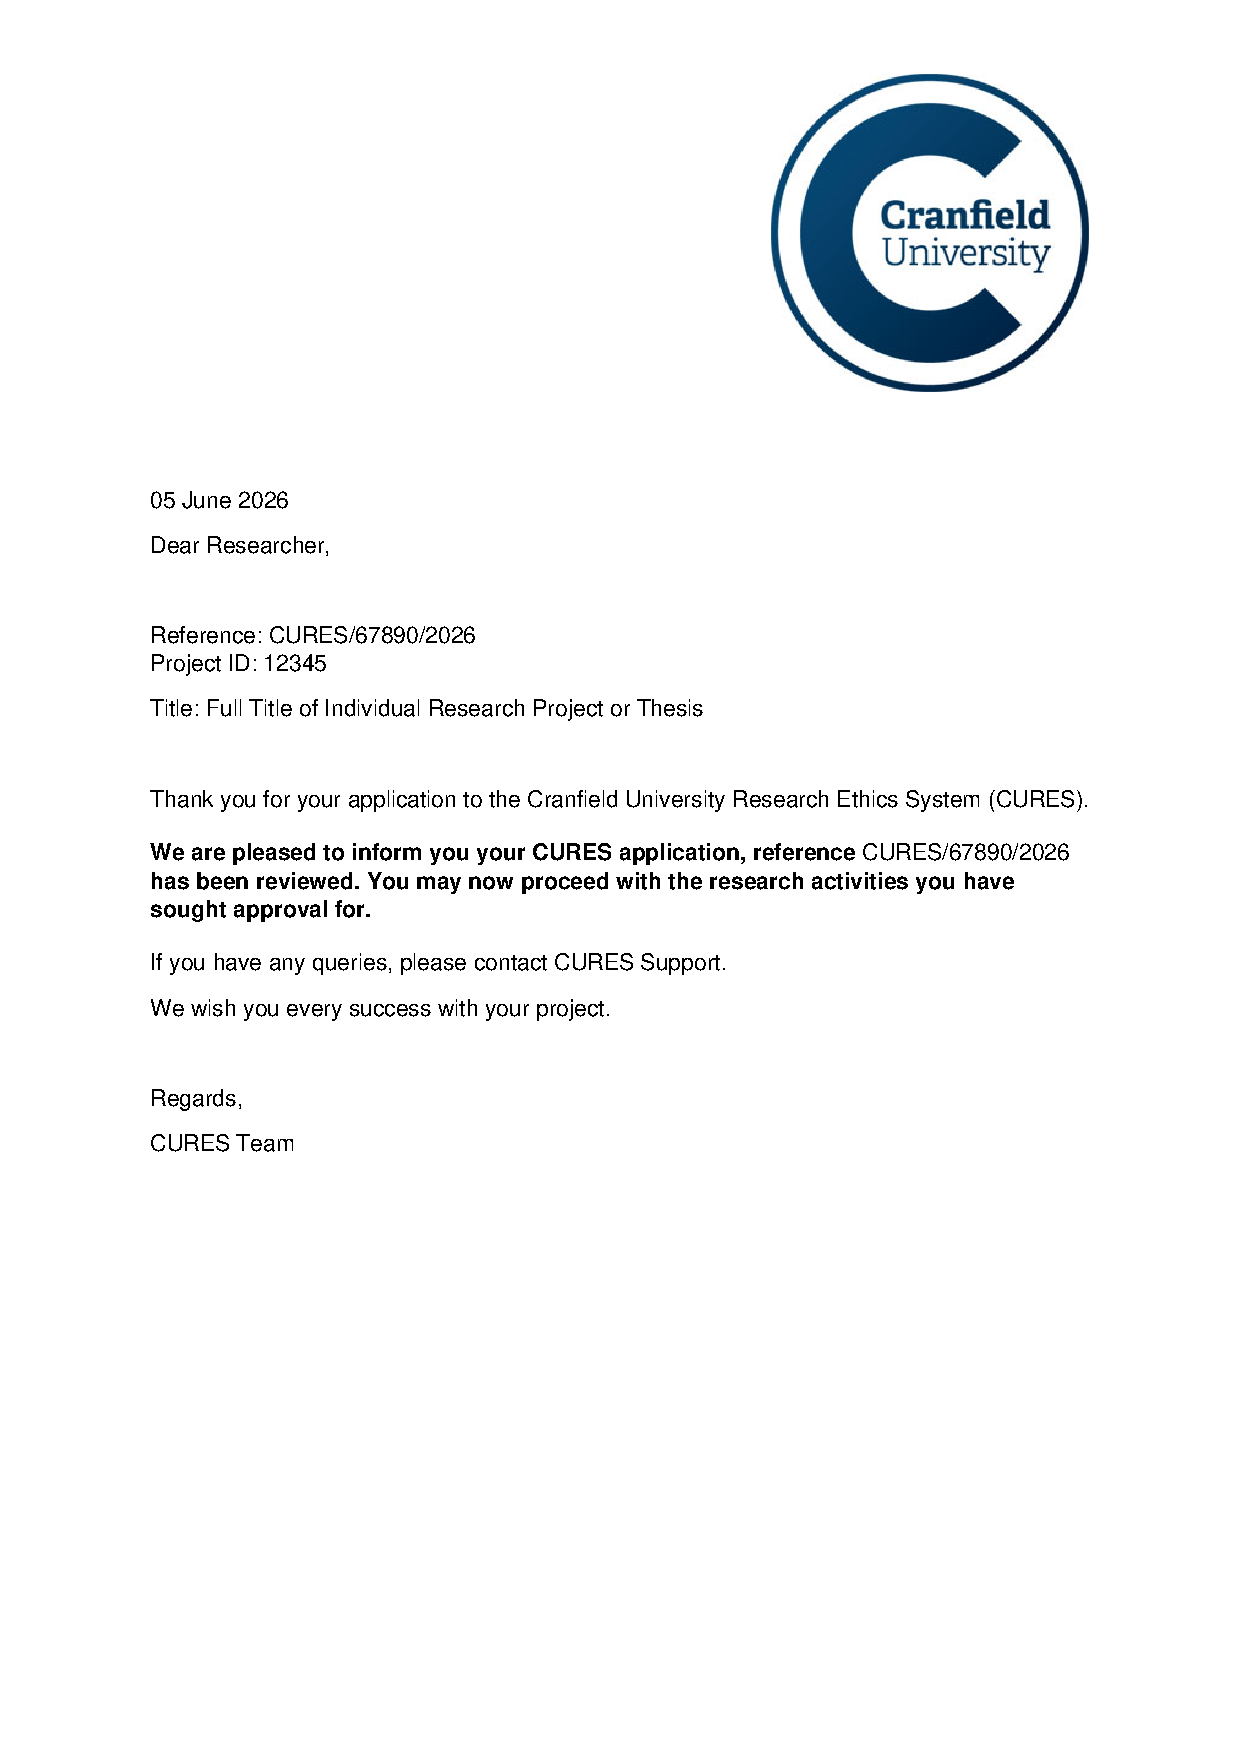
\includegraphics[width=0.9\textwidth, trim={1cm 12cm 1cm 0.5cm}, clip,
        alt={The ethical approval letter from the CURES system.}]{Letter.pdf}
\end{figure}

\chapter{Implementation Details}\label{app:Implementation}
This appendix collects implementation details for reproducibility.

\section{Software and hardware}
\begin{itemize}
    \item Simulator: MuJoCo~3.9 (EGL offscreen rendering).
    \item Learning framework: Hugging Face LeRobot \parencite{cadene2024lerobot};
    policy \texttt{smolvla\_base}.
    \item Inverse kinematics: \texttt{mink} (MuJoCo-native differential IK).
    \item Assets: robosuite grocery and Omron meshes; UR10e and Robotiq 2F-85 from
    the MuJoCo Menagerie.
    \item Hardware: NVIDIA RTX~A2000 (12~GB).
\end{itemize}

\section{Training hyper-parameters}
\begin{table}[ht]
\caption{SmolVLA fine-tuning configuration.}
\begin{center}
\tagpdfsetup{table/header-rows={1}}
\begin{tabular}{ll}
\toprule
Setting & Value \\
\midrule
Base checkpoint & \texttt{smolvla\_base} \\
Backbone & Frozen (action expert trained) \\
Batch size & 8 \\
Optimisation steps & 20{,}000 \\
Checkpoints saved & every 5{,}000 steps (5k/10k/15k/20k) \\
Action chunk length & 50 \\
Wall-clock training time & $\approx$ 4 hours \\
Peak GPU memory & $\approx$ 3~GB \\
\bottomrule
\end{tabular}
\end{center}
\label{tab:hyperparams}
\end{table}

\section{Dataset}
\begin{itemize}
    \item 240 successful demonstrations (60 per item $\times$ 4 items:
    cola can, water bottle, milk carton, bread loaf).
    \item Per step: three RGB images ($96\times96$; wrist, scene, basket), 7-D state
    (6 arm joints + gripper), 7-D action, and a language instruction.
    \item $\approx$ 20 instruction paraphrases; per-episode positional jitter.
    \item Recorded at 100~Hz, subsampled $5\times$ to 20~fps; LeRobot dataset format
    (parquet + video); per-item validation hold-out.
    \item Demonstrations end at placement (clean episode boundary).
\end{itemize}

\section{Evaluation protocol}
\begin{itemize}
    \item Closed-loop rollouts at $\approx$ 20~Hz; actions applied directly.
    \item Metrics: grasp success (item lifted clear of the shelf) and task
    completion (item at rest inside the basket footprint).
    \item $\geq 20$ trials per item; fresh seeds and paraphrases per trial.
    \item Wilson 95\% confidence intervals \parencite{wilson1927ci}.
    \item Checkpoint selected by closed-loop task success; normalisation statistics
    loaded from the same checkpoint.
    \item Multi-checkpoint evaluation: 4 checkpoints $\times$ 4 items $\times$ 20
    trials $=$ 320 rollouts.
\end{itemize}

\section{Software pipeline and reproducibility}
The pipeline is organised as a sequence of small, single-purpose scripts so that each
stage can be run and verified independently:
\begin{itemize}
    \item \texttt{envs/supermarket\_env.py} --- builds the MuJoCo model
    programmatically and exposes stepping, rendering and introspection helpers.
    \item \texttt{find\_grasp.py} --- \texttt{mink} inverse-kinematics solvers for grasp
    and place poses.
    \item \texttt{scripted\_expert.py} --- the scripted pick-and-place trajectory and
    the demonstration recorder hook.
    \item \texttt{collect\_data.py} / \texttt{convert\_to\_lerobot.py} --- demonstration
    collection and conversion to the LeRobot dataset format.
    \item \texttt{rollout.py} / \texttt{eval\_checkpoints.py} --- closed-loop evaluation
    and multi-checkpoint success reporting with Wilson intervals.
    \item \texttt{shopping\_list.py} --- the menu-driven multi-item orchestrator.
\end{itemize}
Headless stages set \texttt{MUJOCO\_GL=egl}; the interactive viewer requires a display
and must not set that variable. Determinism is controlled per-trial by an explicit
random seed; because the policy is stochastic, aggregate metrics rather than single
seeds are the unit of reporting.

\section{Coordinate conventions}
All positions in the main text are given in the robot base frame (metres): $x$ points
from the base toward the shelf, $y$ is lateral (positive toward the water bottle,
negative toward the milk carton), and $z$ is vertical. The five products rest along the
shelf front at $y\in\{-0.26,-0.13,0.00,0.15,0.34\}$ and the basket centre is at
approximately $(0.24,0.00)$.


\end{document}
